\documentclass[10pt,conference]{IEEEtran}
\usepackage[hidelinks]{hyperref}
%\documentclass[twocolumn]{article}
\usepackage{verbatim}
\usepackage[utf8x]{inputenc}
\usepackage[a4paper,margin=1.4cm]{geometry}
\usepackage[fleqn]{amsmath}
\usepackage{mathpartir}
\usepackage{amssymb}
\usepackage[makeroom]{cancel}
\usepackage{graphicx}
\usepackage{authblk}

% \usepackage{minted}
\title{A semantics of core AUTOSAR}
\author{Johan Nordlander \quad\quad Patrik Jansson}


\affil{Department of Computer Science and Engineering, Chalmers University of Technology}

%%%%%%%
\newcommand{\sep}{\hspace{2ex}|\hspace{2ex}}


%----------------
%\newcommand{\V}[1]{\textit{\lowercase{#1}}}
\newcommand{\V}[1]{\ensuremath{\lowercase{#1}}}
%{ Not used in semantics.tex
\newcommand{\Code} {\V{Code}}
\newcommand{\Cont} {\V{Cont}}  %TODO: Sometimes just K is used - check for consistency.
\newcommand{\State}{\V{State}}
\newcommand{\Act}  {\V{Act}}
\newcommand{\Upd}  {\V{Upd}}
\newcommand{\Xs}   {\V{Xs}}
\newcommand{\Vs}   {\V{Vs}}
\newcommand{\Cs}   {\V{Cs}}
%}

\newcommand{\kw}[1]{\textbf{#1}}
\newcommand{\Tserving} [2]{\kw{serving}(#1,#2)}

\newcommand{\Trunnable}[5]{\kw{runnable}(#1,#2,#3,#4,#5)}
\newcommand{\Trinst}   [4]{\kw{rinst}(#1,#2,#3,#4)}
\newcommand{\Texcl}    [2]{\kw{excl}(#1,#2)}
\newcommand{\Tirv}     [2]{\kw{irv}(#1,#2)}
\newcommand{\Tdelem}   [3]{\kw{delem}(#1,#2,#3)}
\newcommand{\Tqelem}   [3]{\kw{qelem}(#1,#2,#3)}
\newcommand{\Topres}   [2]{\kw{opres}(#1,#2)}
\newcommand{\Ttimer}   [2]{\kw{timer}(#1,#2)}

%TODO: start with lower case
\newcommand{\rte}[1]{\text{#1}}
%\newcommand{\rte}[1]{\text{rte\_#1}}
\newcommand{\Enter}     [2]{\rte{enter}(#1,#2)}
\newcommand{\Exit}      [2]{\rte{exit}(#1,#2)}
\newcommand{\IrvWrite}  [3]{\rte{irvWrite}(#1,#2,#3)}
\newcommand{\IrvRead}   [2]{\rte{irvRead}(#1,#2)}
\newcommand{\Send}      [3]{\rte{send}(#1,#2,#3)}
\newcommand{\Receive}   [2]{\rte{receive}(#1,#2)}
\newcommand{\Write}     [3]{\rte{write}(#1,#2,#3)}
\newcommand{\Read}      [2]{\rte{read}(#1,#2)}
\newcommand{\Invalidate}[2]{\rte{invalidate}(#1,#2)}
\newcommand{\IsUpdated} [2]{\rte{isUpdated}(#1,#2)}
\newcommand{\Call}      [3]{\rte{call}(#1,#2,#3)}
\newcommand{\Result}    [2]{\rte{result}(#1,#2)}

\newcommand{\Return}    [1]{\text{return}(#1)}

\newcommand{\red} [1]{\,\xrightarrow{#1}\,}
\newcommand{\say} [2]{\ensuremath{#1 \,!\, #2}}
%\newcommand{\say}  [2]{#1\mathrel{\,!\,}#2}
\newcommand{\hear}[2]{\ensuremath{#1 \,?\, #2}}

% ----------------------------------------------------------------

\newcommand{\plusplus}{\mathbin{+\!\!+}}

\newcommand{\Tvar}  [1]{\V{#1}}
\newcommand{\Tatom} [1]{\text{#1}}

\newcommand{\Tpending}      {\kw{pending}}
\newcommand{\Tidle}         {\kw{idle}}



%\newcommand{\Trte}[1]{\mathrm{rte\_#1}}
%\newcommand{\Trte}[2]{\mathrm{#1}#2}
\newcommand{\TrteEnter}     {\Enter}
\newcommand{\TrteExit}      {\Exit}
\newcommand{\TrteIrvWrite}  {\IrvWrite}
\newcommand{\TrteIrvRead}   {\IrvRead}
\newcommand{\TrteSend}      {\Send}
\newcommand{\TrteReceive}   {\Receive}
\newcommand{\TrteWrite}     {\Write}
\newcommand{\TrteRead}      {\Read}
\newcommand{\TrteInvalidate}{\Invalidate}
\newcommand{\TrteIsUpdated} {\IsUpdated}
\newcommand{\TrteCall}      {\Call}
\newcommand{\TrteResult}    {\Result}

\newcommand{\Treturn}       {\Return}

\newcommand{\Tstep}      [3]{\ensuremath{#1 &\red{#2}& #3}}
\newcommand{\Tsay}          {\say}
\newcommand{\Thear}         {\hear}
\newcommand{\Tdelta}     [1]{\ensuremath{\delta(#1)}}

\newcommand{\Tok}           {\Tatom{ok}}
\newcommand{\Tfree}         {\Tatom{free}}
\newcommand{\Ttaken}        {\Tatom{taken}}
\newcommand{\Teps}          {\epsilon}
\newcommand{\Tnodata}       {\Tatom{nodata}}
\newcommand{\Tlimit}        {\Tatom{limit}}
\newcommand{\Tfalse}        {\Tatom{false}}
\newcommand{\Ttrue}         {\Tatom{true}}
\newcommand{\Tinvalid}      {\Tatom{invalid}}
\newcommand{\Tnil}          {\kw{nil}}
\newcommand{\Tvoid}         {\Tatom{void}}
\newcommand{\Tenter}        {\Tatom{enter}}
\newcommand{\Texit}         {\Tatom{exit}}
\newcommand{\Tinv}          {\Tatom{inv}}
\newcommand{\Tterm}         {\Tatom{term}}
\newcommand{\Tnull}         {\Tatom{null}}
\newcommand{\Tnew}          {\Tatom{new}}
\newcommand{\Ttick}         {\Tatom{tick}}

% ----------------

%\newcommand{\Pif}{\ensuremath{\mathbin{:\!\!-}}}
\newcommand{\Pif}{\text{if}}

\newcommand{\Prule}[2]{#1 \\ & & \Pif \;\; #2\\}
%\newcommand{\Pcontline}[1]{\\\multicolumn{3}{l}{\qquad #1}}
\newcommand{\Pcontline}[1]{\\ #1}
\newcommand{\PruleLong}[2]{#1 \Pcontline{&&\Pif \;\; #2.}\\}
\newcommand{\Pfact}[1]{#1.\\}
\newcommand{\Pnegate}[1]{\neg(#1)}

\newcommand{\Opar}{\ensuremath{\mathbin{\,|\,}}}
\newcommand{\Tpar}    [2]{#1 \Opar #2}
\newcommand{\TparLong}[2]{\begin{array}{@{}l} ~~#1 \\ \Opar #2 \end{array}}

%\newcommand{\Tr}    [2]{\mathrm{r}(#1,#2)}
%\newcommand{\Tx}    [2]{\mathrm{x}(#1,#2)}
%\newcommand{\Ts}    [2]{\mathrm{s}(#1,#2)}
\newcommand{\Tr}    [2]{\emph{#2.#1}}
\newcommand{\Tx}    [2]{\emph{#2.#1}}
\newcommand{\Ts}    [2]{\emph{#2.#1}}
\newcommand{\Te}    [2]{\emph{#2.#1}}
\newcommand{\To}    [2]{\emph{#2.#1}}
\newcommand{\Tep}   [3]{\emph{#3.#2.#1}}
\newcommand{\Top}   [3]{\emph{#3.#2.#1}}

%\newcommand{\Tcons}         [2]{\mathrm{cons}(#1,#2)}
\newcommand{\Tcons}         [2]{#1:#2}
\newcommand{\Tap}           [2]{#1(#2)}
%\newcommand{\Tseq}          [2]{#1\mathbin{\plusplus}#2}
\newcommand{\Tsnoc}{\Tseq}
\newcommand{\Tseq}          [2]{#1{:}#2}

\newcommand{\Tasyncresult}  [1]{\mathrm{async\_result}(#1)}
\newcommand{\Tasync}        [1]{\mathrm{async}(#1)}
\newcommand{\Tsync}         [1]{\mathrm{sync}(#1)}
%\newcommand{\Tconnect}      [2]{\mathrm{connect}(#1,#2)}
\newcommand{\Tconnect}      [2]{\ensuremath{#1 \Rightarrow #2}}
\newcommand{\Tevents}       [1]{\mathrm{events}(#1)}

%%% static properties
\newcommand{\TcanBeInvokedConcurrently}    [1]{\mathrm{canBeInvokedConcurrently}(#1)}
\newcommand{\TminimumStartInterval}        [2]{\mathrm{minimumStartInterval}(#1,#2)}
\newcommand{\TdataReceived}                [1]{\mathrm{dataReceived}(#1)}

\newcommand{\ToperationInvoked}[1]{\mathrm{operationInvoked}(#1)}

\newcommand{\TserverCallPoint}[1]{\mathrm{serverCallPoint}(#1)}
\newcommand{\Ttiming}       [1]{\mathrm{timing}(#1)}


%%% operators
\newcommand{\Tless}         [2]{#1<#2}
\newcommand{\Tlesseq}       [2]{#1 \leq #2}
\newcommand{\Tminus}        [2]{{#1}-{#2}}
\newcommand{\Tplus}         [2]{{#1}+{#2}}
\newcommand{\Tequal}        [2]{{#1}={#2}}
\newcommand{\Tmember}       [2]{#1 \in #2}
\newcommand{\Tlength}       [1]{|#1|}

%%% payload
\newcommand{\Tcall}         [2]{\mathrm{call}(#1,#2)}
\newcommand{\Tsnd}          [2]{\mathrm{snd}(#1,#2)}
\newcommand{\Tirvr}         [1]{\mathrm{irvr}(\!#1)}
\newcommand{\Tirvw}         [1]{\mathrm{irvw}(#1)}
\newcommand{\Trcv}          [1]{\mathrm{rcv}(#1)}
\newcommand{\Trd}           [1]{\mathrm{rd}(#1)}
\newcommand{\Twr}           [1]{\mathrm{wr}(#1)}
\newcommand{\Tres}          [1]{\mathrm{res}(#1)}
\newcommand{\Tret}          [1]{\mathrm{ret}(#1)}
\newcommand{\Tup}           [1]{\mathrm{up}(#1)}

\newcommand{\CombRed}{%
\Prule{\Tstep{\Tpar{\Tvar{P_1}}{\Tvar{Q_1}}}{\Tsay{\Tvar{A}}{\Tvar{L}}}{\Tpar{\Tvar{P_2}}{\Tvar{Q_2}}}}{\Tstep{\Tvar{P_1}}{\Tsay{\Tvar{A}}{\Tvar{L}}}{\Tvar{P_2}},\Tstep{\Tvar{Q_1}}{\Thear{\Tvar{A}}{\Tvar{L}}}{\Tvar{Q_2}}}
\Prule{\Tstep{\Tpar{\Tvar{P_1}}{\Tvar{Q_1}}}{\Tsay{\Tvar{A}}{\Tvar{L}}}{\Tpar{\Tvar{P_2}}{\Tvar{Q_2}}}}{\Tstep{\Tvar{P_1}}{\Thear{\Tvar{A}}{\Tvar{L}}}{\Tvar{P_2}},\Tstep{\Tvar{Q_1}}{\Tsay{\Tvar{A}}{\Tvar{L}}}{\Tvar{Q_2}}}
\Prule{\Tstep{\Tpar{\Tvar{P_1}}{\Tvar{Q_1}}}{\Thear{\Tvar{A}}{\Tvar{L}}}{\Tpar{\Tvar{P_2}}{\Tvar{Q_2}}}}{\Tstep{\Tvar{P_1}}{\Thear{\Tvar{A}}{\Tvar{L}}}{\Tvar{P_2}},\Tstep{\Tvar{Q_1}}{\Thear{\Tvar{A}}{\Tvar{L}}}{\Tvar{Q_2}}}
\Prule{\Tstep{\Tpar{\Tvar{P_1}}{\Tvar{Q_1}}}{\Tdelta{\Tvar{T}}}{\Tpar{\Tvar{P_2}}{\Tvar{Q_2}}}}{\Tstep{\Tvar{P_1}}{\Tdelta{\Tvar{T}}}{\Tvar{P_2}},\Tstep{\Tvar{Q_1}}{\Tdelta{\Tvar{T}}}{\Tvar{Q_2}}}
}
\newcommand{\ExclusiveAreas}{%
\Pfact{\Tstep{\Trinst{\Tr{\Tvar{R}}{\Tvar{I}}}{\Tvar{C}}{\Tvar{Xs}}{\TrteEnter{\Tvar{X}}{\Tvar{K}}}}{\Tsay{\Tx{\Tvar{X}}{\Tvar{I}}}{\Tenter}}{\Trinst{\Tr{\Tvar{R}}{\Tvar{I}}}{\Tvar{C}}{\Tcons{\Tvar{X}}{\Tvar{Xs}}}{\Tap{\Tvar{K}}{\Tok}}}}
\Pfact{\Tstep{\Trinst{\Tr{\Tvar{R}}{\Tvar{I}}}{\Tvar{C}}{\Tcons{\Tvar{X}}{\Tvar{Xs}}}{\TrteExit{\Tvar{X}}{\Tvar{K}}}}{\Tsay{\Tx{\Tvar{X}}{\Tvar{I}}}{\Texit}}{\Trinst{\Tr{\Tvar{R}}{\Tvar{I}}}{\Tvar{C}}{\Tvar{Xs}}{\Tap{\Tvar{K}}{\Tok}}}}
\Pfact{\Tstep{\Texcl{\Tx{\Tvar{X}}{\Tvar{I}}}{\Tfree}}{\Thear{\Tx{\Tvar{X}}{\Tvar{I}}}{\Tenter}}{\Texcl{\Tx{\Tvar{X}}{\Tvar{I}}}{\Ttaken}}}
\Pfact{\Tstep{\Texcl{\Tx{\Tvar{X}}{\Tvar{I}}}{\Ttaken}}{\Thear{\Tx{\Tvar{X}}{\Tvar{I}}}{\Texit}}{\Texcl{\Tx{\Tvar{X}}{\Tvar{I}}}{\Tfree}}}
}
\newcommand{\InterrunnableVariables}{%
\Pfact{\Tstep{\Trinst{\Tr{\Tvar{R}}{\Tvar{I}}}{\Tvar{C}}{\Tvar{Xs}}{\TrteIrvRead{\Tvar{S}}{\Tvar{K}}}}{\Tsay{\Ts{\Tvar{S}}{\Tvar{I}}}{\Tirvr{\Tvar{V}}}}{\Trinst{\Tr{\Tvar{R}}{\Tvar{I}}}{\Tvar{C}}{\Tvar{Xs}}{\Tap{\Tvar{K}}{\Tvar{V}}}}}
\Pfact{\Tstep{\Trinst{\Tr{\Tvar{R}}{\Tvar{I}}}{\Tvar{C}}{\Tvar{Xs}}{\TrteIrvWrite{\Tvar{S}}{\Tvar{V}}{\Tvar{K}}}}{\Tsay{\Ts{\Tvar{S}}{\Tvar{I}}}{\Tirvw{\Tvar{V}}}}{\Trinst{\Tr{\Tvar{R}}{\Tvar{I}}}{\Tvar{C}}{\Tvar{Xs}}{\Tap{\Tvar{K}}{\Tok}}}}
\Pfact{\Tstep{\Tirv{\Ts{\Tvar{S}}{\Tvar{I}}}{\Tvar{V}}}{\Thear{\Ts{\Tvar{S}}{\Tvar{I}}}{\Tirvr{\Tvar{V}}}}{\Tirv{\Ts{\Tvar{S}}{\Tvar{I}}}{\Tvar{V}}}}
\Pfact{\Tstep{\Tirv{\Ts{\Tvar{S}}{\Tvar{I}}}{\_}}{\Thear{\Ts{\Tvar{S}}{\Tvar{I}}}{\Tirvw{\Tvar{V}}}}{\Tirv{\Ts{\Tvar{S}}{\Tvar{I}}}{\Tvar{V}}}}
}
\newcommand{\SendingReceiving}{%
\Pfact{\Tstep{\Trinst{\Tr{\Tvar{R}}{\Tvar{I}}}{\Tvar{C}}{\Tvar{Xs}}{\TrteReceive{\Te{\Tvar{E}}{\Tvar{P}}}{\Tvar{K}}}}{\Tsay{\Tep{\Tvar{E}}{\Tvar{P}}{\Tvar{I}}}{\Trcv{\Tvar{V}}}}{\Trinst{\Tr{\Tvar{R}}{\Tvar{I}}}{\Tvar{C}}{\Tvar{Xs}}{\Tap{\Tvar{K}}{\Tvar{V}}}}}
\Pfact{\Tstep{\Trinst{\Tr{\Tvar{R}}{\Tvar{I}}}{\Tvar{C}}{\Tvar{Xs}}{\TrteSend{\Te{\Tvar{E}}{\Tvar{P}}}{\Tvar{V}}{\Tvar{K}}}}{\Tsay{\Tep{\Tvar{E}}{\Tvar{P}}{\Tvar{I}}}{\Tsnd{\Tvar{V}}{\Tvar{Res}}}}{\Trinst{\Tr{\Tvar{R}}{\Tvar{I}}}{\Tvar{C}}{\Tvar{Xs}}{\Tap{\Tvar{K}}{\Tvar{Res}}}}}
\Pfact{\Tstep{\Tqelem{\Tep{\Tvar{E}}{\Tvar{P}}{\Tvar{I}}}{\Tvar{N}}{\Tcons{\Tvar{V}}{\Tvar{Vs}}}}{\Thear{\Tep{\Tvar{E}}{\Tvar{P}}{\Tvar{I}}}{\Trcv{\Tvar{V}}}}{\Tqelem{\Tep{\Tvar{E}}{\Tvar{P}}{\Tvar{I}}}{\Tvar{N}}{\Tvar{Vs}}}}
\Pfact{\Tstep{\Tqelem{\Tep{\Tvar{E}}{\Tvar{P}}{\Tvar{I}}}{\Tvar{N}}{\Teps}}{\Thear{\Tep{\Tvar{E}}{\Tvar{P}}{\Tvar{I}}}{\Trcv{\Tnodata}}}{\Tqelem{\Tep{\Tvar{E}}{\Tvar{P}}{\Tvar{I}}}{\Tvar{N}}{\Teps}}}
\Prule{\Tstep{\Tqelem{\Tep{\Tvar{E}}{\Tvar{P}}{\Tvar{I}}}{\Tvar{N}}{\Tvar{Vs}}}{\Thear{\Tvar{A}}{\Tsnd{\Tvar{V}}{\Tok}}}{\Tqelem{\Tep{\Tvar{E}}{\Tvar{P}}{\Tvar{I}}}{\Tvar{N}}{\Tseq{\Tvar{Vs}}{\Tvar{V}}}}}{\Tconnect{\Tvar{A}}{\Tep{\Tvar{E}}{\Tvar{P}}{\Tvar{I}}},\Tless{\Tlength{\Tvar{Vs}}}{\Tvar{N}}}
\Prule{\Tstep{\Tqelem{\Tep{\Tvar{E}}{\Tvar{P}}{\Tvar{I}}}{\Tvar{N}}{\Tvar{Vs}}}{\Thear{\Tvar{A}}{\Tsnd{\_}{\Tlimit}}}{\Tqelem{\Tep{\Tvar{E}}{\Tvar{P}}{\Tvar{I}}}{\Tvar{N}}{\Tvar{Vs}}}}{\Tconnect{\Tvar{A}}{\Tep{\Tvar{E}}{\Tvar{P}}{\Tvar{I}}},\Tequal{\Tlength{\Tvar{Vs}}}{\Tvar{N}}}
\Prule{\Tstep{\Tqelem{\Tep{\Tvar{E}}{\Tvar{P}}{\Tvar{I}}}{\Tvar{N}}{\Tvar{Vs}}}{\Thear{\Tvar{A}}{\Tsnd{\Tvar{V}}{\Tlimit}}}{\Tqelem{\Tep{\Tvar{E}}{\Tvar{P}}{\Tvar{I}}}{\Tvar{N}}{\Tseq{\Tvar{Vs}}{\Tvar{V}}}}}{\Tconnect{\Tvar{A}}{\Tep{\Tvar{E}}{\Tvar{P}}{\Tvar{I}}},\Tless{\Tlength{\Tvar{Vs}}}{\Tvar{N}}}
\Prule{\Tstep{\Trunnable{\Tr{\Tvar{R}}{\Tvar{I}}}{\Tvar{K}}{\Tvar{T}}{\_}{\Tvar{N}}}{\Thear{\Tvar{A}}{\Tsnd{\_}{\Tok}}}{\Trunnable{\Tr{\Tvar{R}}{\Tvar{I}}}{\Tvar{K}}{\Tvar{T}}{\Tpending}{\Tvar{N}}}}{\Tconnect{\Tvar{A}}{\Tep{\Tvar{E}}{\Tvar{P}}{\Tvar{I}}},\Tmember{\TdataReceived{\Te{\Tvar{E}}{\Tvar{P}}}}{\Tevents{\Tr{\Tvar{R}}{\Tvar{I}}}}}
\Prule{\Tstep{\Trunnable{\Tr{\Tvar{R}}{\Tvar{I}}}{\Tvar{K}}{\Tvar{T}}{\Tvar{Act}}{\Tvar{N}}}{\Thear{\Tvar{A}}{\Tsnd{\_}{\Tlimit}}}{\Trunnable{\Tr{\Tvar{R}}{\Tvar{I}}}{\Tvar{K}}{\Tvar{T}}{\Tvar{Act}}{\Tvar{N}}}}{\Tconnect{\Tvar{A}}{\Tep{\Tvar{E}}{\Tvar{P}}{\Tvar{I}}},\Tmember{\TdataReceived{\Te{\Tvar{E}}{\Tvar{P}}}}{\Tevents{\Tr{\Tvar{R}}{\Tvar{I}}}}}
}
\newcommand{\ReadingWriting}{%
\Pfact{\Tstep{\Trinst{\Tr{\Tvar{R}}{\Tvar{I}}}{\Tvar{C}}{\Tvar{Xs}}{\TrteRead{\Te{\Tvar{E}}{\Tvar{P}}}{\Tvar{K}}}}{\Tsay{\Tep{\Tvar{E}}{\Tvar{P}}{\Tvar{I}}}{\Trd{\Tvar{V}}}}{\Trinst{\Tr{\Tvar{R}}{\Tvar{I}}}{\Tvar{C}}{\Tvar{Xs}}{\Tap{\Tvar{K}}{\Tvar{V}}}}}
\Pfact{\Tstep{\Trinst{\Tr{\Tvar{R}}{\Tvar{I}}}{\Tvar{C}}{\Tvar{Xs}}{\TrteWrite{\Te{\Tvar{E}}{\Tvar{P}}}{\Tvar{V}}{\Tvar{K}}}}{\Tsay{\Tep{\Tvar{E}}{\Tvar{P}}{\Tvar{I}}}{\Twr{\Tvar{V}}}}{\Trinst{\Tr{\Tvar{R}}{\Tvar{I}}}{\Tvar{C}}{\Tvar{Xs}}{\Tap{\Tvar{K}}{\Tok}}}}
\Pfact{\Tstep{\Tdelem{\Tep{\Tvar{E}}{\Tvar{P}}{\Tvar{I}}}{\_}{\Tvar{V}}}{\Thear{\Tep{\Tvar{E}}{\Tvar{P}}{\Tvar{I}}}{\Trd{\Tvar{V}}}}{\Tdelem{\Tep{\Tvar{E}}{\Tvar{P}}{\Tvar{I}}}{\Tfalse}{\Tvar{V}}}}
\Prule{\Tstep{\Tdelem{\Tep{\Tvar{E}}{\Tvar{P}}{\Tvar{I}}}{\_}{\_}}{\Thear{\Tvar{A}}{\Twr{\Tvar{V}}}}{\Tdelem{\Tep{\Tvar{E}}{\Tvar{P}}{\Tvar{I}}}{\Ttrue}{\Tvar{V}}}}{\Tconnect{\Tvar{A}}{\Tep{\Tvar{E}}{\Tvar{P}}{\Tvar{I}}}}
\Prule{\Tstep{\Trunnable{\Tr{\Tvar{R}}{\Tvar{I}}}{\Tvar{K}}{\Tvar{T}}{\_}{\Tvar{N}}}{\Thear{\Tvar{A}}{\Twr{\_}}}{\Trunnable{\Tr{\Tvar{R}}{\Tvar{I}}}{\Tvar{K}}{\Tvar{T}}{\Tpending}{\Tvar{N}}}}{\Tconnect{\Tvar{A}}{\Tep{\Tvar{E}}{\Tvar{P}}{\Tvar{I}}},\Tmember{\TdataReceived{\Te{\Tvar{E}}{\Tvar{P}}}}{\Tevents{\Tr{\Tvar{R}}{\Tvar{I}}}}}
\Pfact{\Tstep{\Trinst{\Tr{\Tvar{R}}{\Tvar{I}}}{\Tvar{C}}{\Tvar{Xs}}{\TrteIsUpdated{\Te{\Tvar{E}}{\Tvar{P}}}{\Tvar{K}}}}{\Tsay{\Tep{\Tvar{E}}{\Tvar{P}}{\Tvar{I}}}{\Tup{\Tvar{U}}}}{\Trinst{\Tr{\Tvar{R}}{\Tvar{I}}}{\Tvar{C}}{\Tvar{Xs}}{\Tap{\Tvar{K}}{\Tvar{U}}}}}
\Pfact{\Tstep{\Trinst{\Tr{\Tvar{R}}{\Tvar{I}}}{\Tvar{C}}{\Tvar{Xs}}{\TrteInvalidate{\Te{\Tvar{E}}{\Tvar{P}}}{\Tvar{K}}}}{\Tsay{\Tep{\Tvar{E}}{\Tvar{P}}{\Tvar{I}}}{\Tinv}}{\Trinst{\Tr{\Tvar{R}}{\Tvar{I}}}{\Tvar{C}}{\Tvar{Xs}}{\Tap{\Tvar{K}}{\Tok}}}}
\Pfact{\Tstep{\Tdelem{\Tep{\Tvar{E}}{\Tvar{P}}{\Tvar{I}}}{\Tvar{U}}{\Tvar{V}}}{\Thear{\Tep{\Tvar{E}}{\Tvar{P}}{\Tvar{I}}}{\Tup{\Tvar{U}}}}{\Tdelem{\Tep{\Tvar{E}}{\Tvar{P}}{\Tvar{I}}}{\Tvar{U}}{\Tvar{V}}}}
\Prule{\Tstep{\Tdelem{\Tep{\Tvar{E}}{\Tvar{P}}{\Tvar{I}}}{\_U}{\_}}{\Thear{\Tvar{A}}{\Tinv}}{\Tdelem{\Tep{\Tvar{E}}{\Tvar{P}}{\Tvar{I}}}{\Ttrue}{\Tinvalid}}}{\Tconnect{\Tvar{A}}{\Tep{\Tvar{E}}{\Tvar{P}}{\Tvar{I}}}}
}
\newcommand{\CallServer}{%
\Prule{\Tstep{\Trinst{\Tr{\Tvar{R}}{\Tvar{I}}}{\Tvar{C}}{\Tvar{Xs}}{\TrteCall{\To{\Tvar{O}}{\Tvar{P}}}{\Tvar{V}}{\Tvar{K}}}}{\Tsay{\Top{\Tvar{O}}{\Tvar{P}}{\Tvar{I}}}{\Tcall{\Tvar{V}}{\Tok}}}{\Trinst{\Tr{\Tvar{R}}{\Tvar{I}}}{\Tvar{C}}{\Tvar{Xs}}{\TrteResult{\To{\Tvar{O}}{\Tvar{P}}}{\Tvar{K}}}}}{\Tmember{\Tsync{\To{\Tvar{O}}{\Tvar{P}}}}{\TserverCallPoint{\Tr{\Tvar{R}}{\Tvar{I}}}}}
\Prule{\Tstep{\Trinst{\Tr{\Tvar{R}}{\Tvar{I}}}{\Tvar{C}}{\Tvar{Xs}}{\TrteCall{\To{\Tvar{O}}{\Tvar{P}}}{\Tvar{V}}{\Tvar{K}}}}{\Tsay{\Top{\Tvar{O}}{\Tvar{P}}{\Tvar{I}}}{\Tcall{\Tvar{V}}{\Tok}}}{\Trinst{\Tr{\Tvar{R}}{\Tvar{I}}}{\Tvar{C}}{\Tvar{Xs}}{\Tap{\Tvar{K}}{\Tvar{Res}}}}}{\Tmember{\Tasync{\To{\Tvar{O}}{\Tvar{P}}}}{\TserverCallPoint{\Tr{\Tvar{R}}{\Tvar{I}}}}}
\Pfact{\Tstep{\Trinst{\Tr{\Tvar{R}}{\Tvar{I}}}{\Tvar{C}}{\Tvar{Xs}}{\TrteCall{\To{\Tvar{O}}{\Tvar{P}}}{\Tvar{V}}{\Tvar{K}}}}{\Tsay{\Top{\Tvar{O}}{\Tvar{P}}{\Tvar{I}}}{\Tcall{\Tvar{V}}{\Tlimit}}}{\Trinst{\Tr{\Tvar{R}}{\Tvar{I}}}{\Tvar{C}}{\Tvar{Xs}}{\Tap{\Tvar{K}}{\Tvar{Res}}}}}
\Prule{\Tstep{\Trunnable{\Tr{\Tvar{R}}{\Tvar{I}}}{\Tvar{K}}{\Tvar{T}}{\Tserving{\Tvar{Cs}}{\Tvar{Vs}}}{\Tvar{N}}}{\Thear{\Tvar{A}}{\Tcall{\Tvar{V}}{\Tok}}}{\Trunnable{\Tr{\Tvar{R}}{\Tvar{I}}}{\Tvar{K}}{\Tvar{T}}{\Tserving{\Tseq{\Tvar{Cs}}{\Tvar{A}}}{\Tseq{\Tvar{Vs}}{\Tvar{V}}}}{\Tvar{N}}}}{\Tconnect{\Tvar{A}}{\Top{\Tvar{O}}{\Tvar{P}}{\Tvar{I}}},\Tmember{\ToperationInvoked{\To{\Tvar{O}}{\Tvar{P}}}}{\Tevents{\Tr{\Tvar{R}}{\Tvar{I}}}},\Pnegate{\Tmember{\Tvar{A}}{\Tvar{Cs}}}}
\Prule{\Tstep{\Trunnable{\Tr{\Tvar{R}}{\Tvar{I}}}{\Tvar{K}}{\Tvar{T}}{\Tserving{\Tvar{Cs}}{\Tvar{Vs}}}{\Tvar{N}}}{\Thear{\Tvar{A}}{\Tcall{\_}{\Tlimit}}}{\Trunnable{\Tr{\Tvar{R}}{\Tvar{I}}}{\Tvar{K}}{\Tvar{T}}{\Tserving{\Tvar{Cs}}{\Tvar{Vs}}}{\Tvar{N}}}}{\Tconnect{\Tvar{A}}{\Top{\Tvar{O}}{\Tvar{P}}{\Tvar{I}}},\Tmember{\ToperationInvoked{\To{\Tvar{O}}{\Tvar{P}}}}{\Tevents{\Tr{\Tvar{R}}{\Tvar{I}}}},\Tmember{\Tvar{A}}{\Tvar{Cs}}}
}
\newcommand{\ServerResult}{%
\Pfact{\Tstep{\Trinst{\Tr{\Tvar{R}}{\Tvar{I}}}{\Tvar{C}}{\Tvar{Xs}}{\TrteResult{\To{\Tvar{O}}{\Tvar{P}}}{\Tvar{K}}}}{\Tsay{\Top{\Tvar{O}}{\Tvar{P}}{\Tvar{I}}}{\Tres{\Tvar{V}}}}{\Trinst{\Tr{\Tvar{R}}{\Tvar{I}}}{\Tvar{C}}{\Tvar{Xs}}{\Tap{\Tvar{K}}{\Tvar{V}}}}}
\Pfact{\Tstep{\Trinst{\Tvar{A}}{\Top{\Tvar{O}}{\Tvar{P}}{\Tvar{I}}}{\Teps}{\Treturn{\Tvar{V}}}}{\Tsay{\Top{\Tvar{O}}{\Tvar{P}}{\Tvar{I}}}{\Tret{\Tvar{V}}}}{\Trinst{\Tvar{A}}{\Tnil}{\Teps}{\Treturn{\Tvoid}}}}
\Pfact{\Tstep{\Topres{\Top{\Tvar{O}}{\Tvar{P}}{\Tvar{I}}}{\Tcons{\Tvar{V}}{\Tvar{Vs}}}}{\Thear{\Top{\Tvar{O}}{\Tvar{P}}{\Tvar{I}}}{\Tres{\Tvar{V}}}}{\Topres{\Top{\Tvar{O}}{\Tvar{P}}{\Tvar{I}}}{\Tvar{Vs}}}}
\Pfact{\Tstep{\Topres{\Top{\Tvar{O}}{\Tvar{P}}{\Tvar{I}}}{\Tvar{Vs}}}{\Thear{\Top{\Tvar{O}}{\Tvar{P}}{\Tvar{I}}}{\Tret{\Tvar{V}}}}{\Topres{\Top{\Tvar{O}}{\Tvar{P}}{\Tvar{I}}}{\Tseq{\Tvar{Vs}}{\Tvar{V}}}}}
\Prule{\Tstep{\Topres{\Top{\Tvar{O}}{\Tvar{P}}{\Tvar{I}}}{\Teps}}{\Thear{\Top{\Tvar{O}}{\Tvar{P}}{\Tvar{I}}}{\Tres{\Tnodata}}}{\Topres{\Top{\Tvar{O}}{\Tvar{P}}{\Tvar{I}}}{\Teps}}}{\Tasyncresult{\Top{\Tvar{O}}{\Tvar{P}}{\Tvar{I}}}}
}
\newcommand{\SpawnTerminate}{%
\Pfact{\Tstep{\Trinst{\Tvar{A}}{\Tnil}{\Teps}{\Treturn{\_}}}{\Tsay{\Tvar{A}}{\Tterm}}{\Tnull}}
\Pfact{\Tstep{\Trunnable{\Tvar{A}}{\Tvar{K}}{\Tvar{T}}{\Tvar{Act}}{\Tvar{N}}}{\Thear{\Tvar{A}}{\Tterm}}{\Trunnable{\Tvar{A}}{\Tvar{K}}{\Tvar{T}}{\Tvar{Act}}{\Tminus{\Tvar{N}}{1}}}}
\Prule{\Tstep{\Trunnable{\Tvar{A}}{\Tvar{K}}{0}{\Tpending}{0}}{\Tsay{\Tvar{A}}{\Tnew}}{\Tpar{\Trunnable{\Tvar{A}}{\Tvar{K}}{\Tvar{T}}{\Tidle}{1}}{\Trinst{\Tvar{A}}{\Tnil}{\Teps}{\Tap{\Tvar{K}}{\Tvoid}}}}}{\TminimumStartInterval{\Tvar{A}}{\Tvar{T}}}
\Prule{\Tstep{\Trunnable{\Tvar{A}}{\Tvar{K}}{0}{\Tpending}{\Tvar{N}}}{\Tsay{\Tvar{A}}{\Tnew}}{\Tpar{\Trunnable{\Tvar{A}}{\Tvar{K}}{\Tvar{T}}{\Tidle}{\Tplus{\Tvar{N}}{1}}}{\Trinst{\Tvar{A}}{\Tnil}{\Teps}{\Tap{\Tvar{K}}{\Tvoid}}}}}{\TcanBeInvokedConcurrently{\Tvar{A}},\TminimumStartInterval{\Tvar{A}}{\Tvar{T}}}
\Prule{\Tstep{\Trunnable{\Tvar{A}}{\Tvar{K}}{0}{\Tserving{\Tcons{\Tvar{C}}{\Tvar{Cs}}}{\Tcons{\Tvar{V}}{\Tvar{Vs}}}}{0}}{\Tsay{\Tvar{A}}{\Tnew}}{\Tpar{\Trunnable{\Tvar{A}}{\Tvar{K}}{\Tvar{T}}{\Tserving{\Tvar{Cs}}{\Tvar{Vs}}}{1}}{\Trinst{\Tvar{A}}{\Tvar{C}}{\Teps}{\Tap{\Tvar{K}}{\Tvar{V}}}}}}{\TminimumStartInterval{\Tvar{A}}{\Tvar{T}}}
\Prule{\Tstep{\Trunnable{\Tvar{A}}{\Tvar{K}}{0}{\Tserving{\Tcons{\Tvar{C}}{\Tvar{Cs}}}{\Tcons{\Tvar{V}}{\Tvar{Vs}}}}{\Tvar{N}}}{\Tsay{\Tvar{A}}{\Tnew}}{\Tpar{\Trunnable{\Tvar{A}}{\Tvar{K}}{\Tvar{T}}{\Tserving{\Tvar{Cs}}{\Tvar{Vs}}}{\Tplus{\Tvar{N}}{1}}}{\Trinst{\Tvar{A}}{\Tvar{C}}{\Teps}{\Tap{\Tvar{K}}{\Tvar{V}}}}}}{\TcanBeInvokedConcurrently{\Tvar{A}},\TminimumStartInterval{\Tvar{A}}{\Tvar{T}}}
}
\newcommand{\PassingTime}{%
\Prule{\Tstep{\Ttimer{\Tvar{A}}{0}}{\Tsay{\Tvar{A}}{\Ttick}}{\Ttimer{\Tvar{A}}{\Tvar{T}}}}{\Tmember{\Tevents{\Tvar{A}}}{\Ttiming{\Tvar{T}}}}
\Pfact{\Tstep{\Trunnable{\Tvar{A}}{\Tvar{K}}{\Tvar{T}}{\_}{\Tvar{N}}}{\Thear{\Tvar{A}}{\Ttick}}{\Trunnable{\Tvar{A}}{\Tvar{K}}{\Tvar{T}}{\Tpending}{\Tvar{N}}}}
\Prule{\Tstep{\Ttimer{\Tvar{A}}{\Tvar{V}}}{\Tdelta{\Tvar{T}}}{\Ttimer{\Tvar{A}}{\Tminus{\Tvar{V}}{\Tvar{T}}}}}{\Tlesseq{\Tvar{T}}{\Tvar{V}}}
\Prule{\Tstep{\Trunnable{\Tvar{A}}{\Tvar{K}}{\Tvar{V}}{\Tvar{Act}}{\Tvar{N}}}{\Tdelta{\Tvar{T}}}{\Trunnable{\Tvar{A}}{\Tvar{K}}{\Tminus{\Tvar{V}}{\Tvar{T}}}{\Tvar{Act}}{\Tvar{N}}}}{\Tlesseq{\Tvar{T}}{\Tvar{V}}}
\Pfact{\Tstep{\Trunnable{\Tvar{A}}{\Tvar{K}}{0}{\Tvar{Act}}{\Tvar{N}}}{\Tdelta{\_}}{\Trunnable{\Tvar{A}}{\Tvar{K}}{0}{\Tvar{Act}}{\Tvar{N}}}}
\Pfact{\Tstep{\Trinst{\Tvar{A}}{\Tvar{C}}{\Tvar{Xs}}{\Tvar{Code}}}{\Tdelta{\_}}{\Trinst{\Tvar{A}}{\Tvar{C}}{\Tvar{Xs}}{\Tvar{Code}}}}
\Pfact{\Tstep{\Texcl{\Tvar{A}}{\Tvar{V}}}{\Tdelta{\_}}{\Texcl{\Tvar{A}}{\Tvar{V}}}}
\Pfact{\Tstep{\Tirv{\Tvar{A}}{\Tvar{V}}}{\Tdelta{\_}}{\Tirv{\Tvar{A}}{\Tvar{V}}}}
\Pfact{\Tstep{\Tqelem{\Tvar{A}}{\Tvar{N}}{\Tvar{Vs}}}{\Tdelta{\_}}{\Tqelem{\Tvar{A}}{\Tvar{N}}{\Tvar{Vs}}}}
\Pfact{\Tstep{\Tdelem{\Tvar{A}}{\Tvar{U}}{\Tvar{V}}}{\Tdelta{\_}}{\Tdelem{\Tvar{A}}{\Tvar{U}}{\Tvar{V}}}}
\Pfact{\Tstep{\Topres{\Tvar{A}}{\Tvar{Vs}}}{\Tdelta{\_}}{\Topres{\Tvar{A}}{\Tvar{Vs}}}}
}
\newcommand{\IgnoreBroadcast}{%
\Pfact{\Tstep{\Trinst{\Tvar{A}}{\Tvar{C}}{\Tvar{Xs}}{\Tvar{K}}}{\Thear{\_}{\_}}{\Trinst{\Tvar{A}}{\Tvar{C}}{\Tvar{Xs}}{\Tvar{K}}}}
\Pfact{\Tstep{\Ttimer{\Tvar{B}}{\Tvar{T}}}{\Thear{\_}{\_}}{\Ttimer{\Tvar{B}}{\Tvar{T}}}}
\Prule{\Tstep{\Trunnable{\Tvar{B}}{\Tvar{K}}{\Tvar{T}}{\Tvar{Act}}{\Tvar{N}}}{\Thear{\Tvar{A}}{\_}}{\Trunnable{\Tvar{B}}{\Tvar{K}}{\Tvar{T}}{\Tvar{Act}}{\Tvar{N}}}}{\Pnegate{\Tequal{\Tvar{A}}{\Tvar{B}}}}
\Prule{\Tstep{\Texcl{\Tvar{B}}{\Tvar{V}}}{\Thear{\Tvar{A}}{\_}}{\Texcl{\Tvar{B}}{\Tvar{V}}}}{\Pnegate{\Tequal{\Tvar{A}}{\Tvar{B}}}}
\Prule{\Tstep{\Tirv{\Tvar{B}}{\Tvar{V}}}{\Thear{\Tvar{A}}{\_}}{\Tirv{\Tvar{B}}{\Tvar{V}}}}{\Pnegate{\Tequal{\Tvar{A}}{\Tvar{B}}}}
\Prule{\Tstep{\Tqelem{\Tvar{B}}{\Tvar{N}}{\Tvar{Vs}}}{\Thear{\Tvar{A}}{\_}}{\Tqelem{\Tvar{B}}{\Tvar{N}}{\Tvar{Vs}}}}{\Pnegate{\Tequal{\Tvar{A}}{\Tvar{B}}},\Pnegate{\Tconnect{\Tvar{A}}{\Tvar{B}}}}
\Prule{\Tstep{\Tdelem{\Tvar{B}}{\Tvar{U}}{\Tvar{V}}}{\Thear{\Tvar{A}}{\_}}{\Tdelem{\Tvar{B}}{\Tvar{U}}{\Tvar{V}}}}{\Pnegate{\Tequal{\Tvar{A}}{\Tvar{B}}},\Pnegate{\Tconnect{\Tvar{A}}{\Tvar{B}}}}
\Prule{\Tstep{\Topres{\Tvar{B}}{\Tvar{Vs}}}{\Thear{\Tvar{A}}{\_}}{\Topres{\Tvar{B}}{\Tvar{Vs}}}}{\Pnegate{\Tequal{\Tvar{A}}{\Tvar{B}}},\Pnegate{\Tconnect{\Tvar{A}}{\Tvar{B}}}}
}


\bibliographystyle{splncs03} % Latest bibtex style for llncs

\setlength{\parindent}{0pt}
\setlength{\parskip}{4pt plus 2pt minus 1pt}

\begin{document}
\maketitle
\begin{abstract}
The AUTOSAR system architecture for the automotive industry is rich in features and large in size, but lacks a comprehensive definition that allows its Software Components and Runtime Environment to be treated as an abstract programming model in its own right. As a result, AUTOSAR components are hard to analyze, test and evaluate without first committing to a particular execution platform and component context. This paper addresses this shortcoming by means of a formalization of the core AUTOSAR specification as a labelled transition system. The resulting semantic rules can be used to clarify the specification, emphasize design tradeoffs and serve as a foundation for tools that fulfill the AUTOSAR promise of platform- and vendor-independent automotive software development.
\end{abstract}

\section{Introduction}
\label{sec:Intro}

The AUTOSAR standard is an open software component architecture for the automotive industry \cite{AR:Homepage}. Its main purpose is to enable interoperability of software modules among different vendors and on heterogeneous platforms, via an extensive set of standardized interfaces and libraries, and a common software development methodology.

The standard has a rather wide scope and covers many features normally associated with complex operating systems, like I/O abstraction, concurrency, communication, distribution and real-time predictability. Unlike existing operating systems, however, AUTOSAR is not de facto defined in terms of a particular implementation. Instead, an explicit goal of AUTOSAR is to constitute an abstract specification that allows multiple and competing realizations, and even systems built as an assembly of fragments from many different (and competing) vendors. Such a goal naturally puts a heavy focus on the standard specification itself.

Unfortunately, the AUTOSAR specification is not very rigorous, despite a sheer size of more than 12,500 pages of text and UML diagrams in total. It is also not very abstract, in that it makes frequent references to assumed implementation techniques for the purpose of defining its semantics. In practice, the AUTOSAR standard becomes blurred with the specific behavior of one's chosen platform and development tools. And because the standard is open to interpretation, the interoperability of software components across tools and platforms is often seriously hampered. What is more, a single software component cannot easily be studied and understood in isolation, since its interactive behavior is only indirectly defined in terms of the concrete C-code and OS tasks that realize it and its interaction environment.

In this paper we take a first step towards a remedy to these problems, by contributing a formal specification of a substantial core of the AUTOSAR standard. AUTOSAR itself is summarized in Section~\ref{sec:autosar}. The formalization covers most of the Software Component Template and its accompanying Run-Time Environment (RTE) (Section~\ref{sec:Calc}), and is able to directly express every legal way a system of software components can evolve at run-time on an arbitrarily fast platform (Section~\ref{sec:Sem}). It can thus serve as a basis for both a concrete AUTOSAR implementation on a specific platform (whose supported behaviors must be a subset of those defined by the formal semantics), and a platform-independent AUTOSAR simulator (where behaviors from the legal set can be picked at random).
Non-determinism and concurrency is emphasized in Section~\ref{sec:NonDet}, together with an example of an unfortunate consequence of the specified standard. Section~\ref{sec:Amb} identifies some areas where the AUTOSAR documents has been found unclear; here our chosen readings are put in relation to alternative interpretations. Section~\ref{sec:Lim}, finally, gives a detailed account on the scope limitations we have imposed on our work.

The semantics has been formalized with the intent to accurately capture the informal meaning of the AUTOSAR standard, although mistakes and misunderstandings are certainly both possible and plausible. A formal notation is nevertheless a good starting point for any discussion on the resolution of such issues. The semantics is furthermore written to be unambiguous, except where concurrent execution should allow for more than one observed behavior. Examples of questions that can be firmly resolved on basis of our formalized semantics include:
\begin{itemize}
\item {\em How many runnable instances will a sequence of received values give rise to?}
\item {\em What values may ever be returned when an inter-runnable variable is first read?}
\item {\em At what times will two timing events coincide, if at all?}
\end{itemize}


\section{AUTOSAR}
\label{sec:autosar}

An AUTOSAR model is primarily a structure of interconnected \textbf{software components} (SWCs) \cite{AR:SWC}. Links between SWCs are called \textbf{connectors}, which attach to \textbf{ports} exposed by the SWCs. A port is either \textbf{required} or \textbf{provided}, and then classified according to what \textbf{interface} it exposes: \textbf{sender-receiver}, \textbf{client-server}, \textbf{trigger} and \textbf{mode-switch} are common interface types. A sender-receiver interface is an aggregation of one or more \textbf{data-elements}, with each element characterized by the type of data it carries and optional further communication specification details. A client-server interface likewise consists of one or more \textbf{operations}, that each gives the signature of a procedure call and the possible errors that may result.

\begin{figure*}
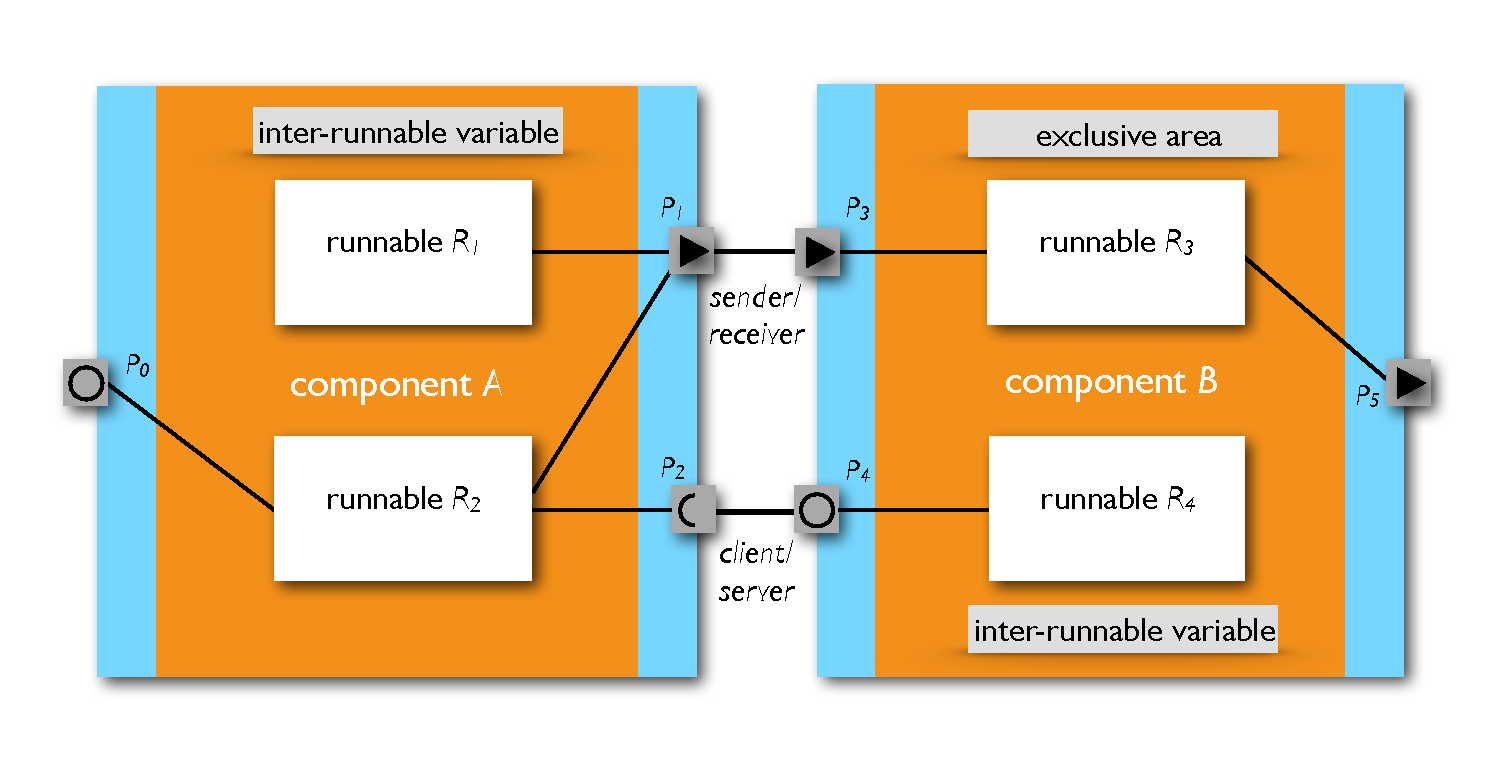
\includegraphics[page=1,width=\textwidth]{Fig}
%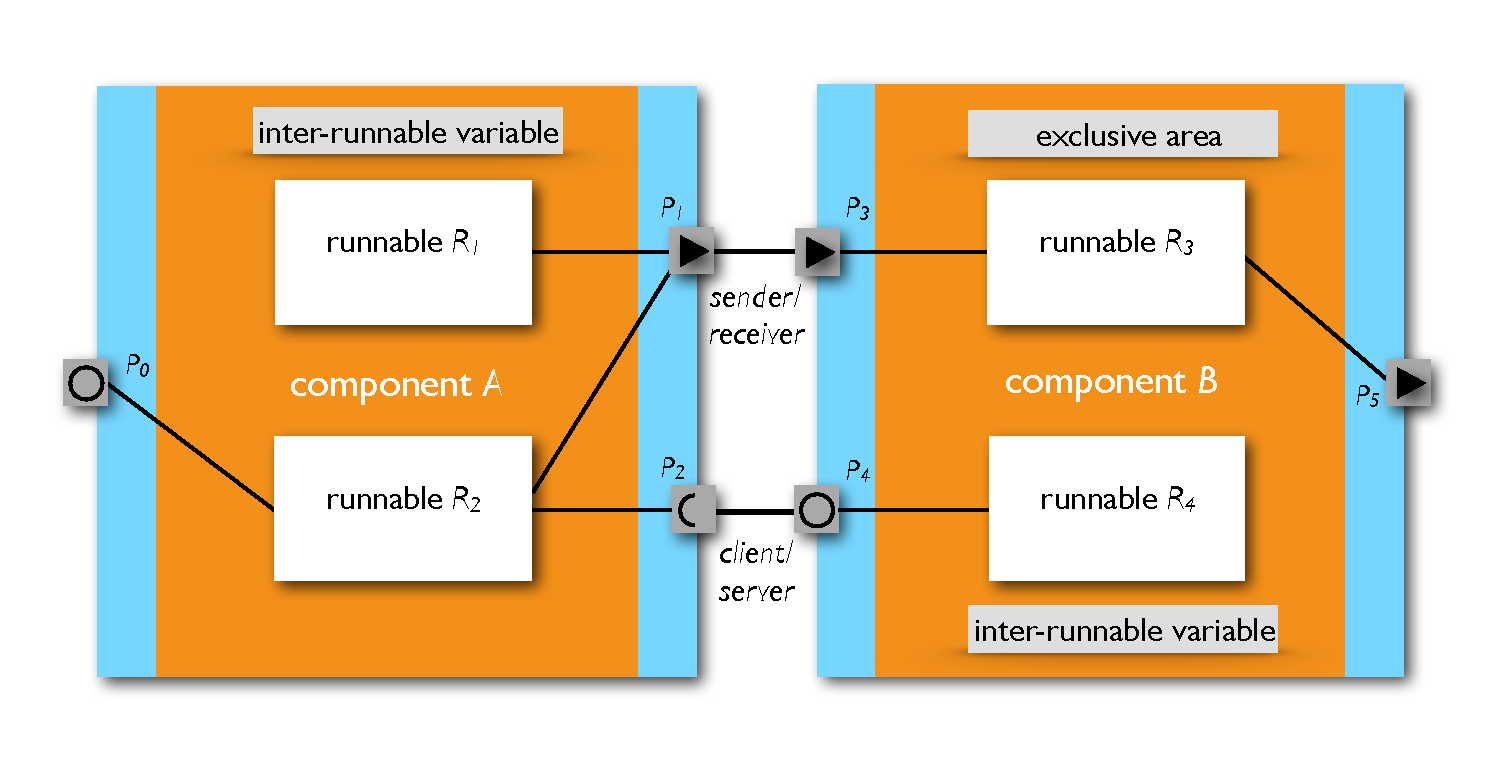
\includegraphics[page=1,scale=0.73]{Fig}
\caption{\label{fig:model}{Example of a graphical AUTOSAR software components model.}}
\end{figure*}


Some components merely act as containers of other components structures, these are called \textbf{composition} SWCs. In contrast, \textbf{atomic} SWCs define their own behavior, primarily in terms of \textbf{runnables} and \textbf{inter-runnable variables}. A runnable denotes a sequential and (normally) terminating piece of code, although its actual behavioral definition is typically relegated to external C or Matlab files rather than being part of the AUTOSAR model proper. Instead, an AUTOSAR runnable only provides constraints on what ports and inter-runnable variables the actual implementation can access; as well as \textbf{event} declarations that determine under what conditions it will get executed.

A runnable under execution is called a \textbf{runnable instance}, and several instances may execute concurrently even if they belong to the same SWC. Each runnable indicates whether or not it may be instantiated concurrently with itself. Runnable code can also use \textbf{exclusive areas} (a form of mutex semaphores) to further control concurrent behavior.

To interact with ports, inter-runnable variables and exclusive areas, runnables use what is abstractly known as the \textbf{virtual function bus} (VFB). Concretely, the VFB takes the shape of a C programming interface to the \textbf{run-time environment} (RTE), custom-generated for each runnable on the basis of its access constraints \cite{AR:RTE}. Behind the RTE, a collection of OS kernels, communication stacks and other basic software modules implement the VFB services for the platform at hand. Complete AUTOSAR designs also typically contain \textbf{ECU} and \textbf{task assignments}, which are manually built tables that control how SWCs and runnables map onto the available hardware and OS resources, respectively.

AUTOSAR models are completely static, which means that all components, runnables, ports, connectors, etc, are created ahead of execution time. Runnable instances are an exception, but they are only identified by AUTOSAR for conceptual purposes and are never part of any model syntax. This static nature renders AUTOSAR models very suitable to graphical notations, which by far is the most widespread representation format for AUTOSAR models. A graphical model example is shown in Figure~\ref{fig:model}.


\section{Syntax and preliminaries}
\label{sec:Calc}

The formal approach we have chosen is that of a typical process calculus \cite{milner:ComMob}, where a system of concurrent processes evolves in a sequence of atomic steps, as determined by a global set of transition rules. Our process terms correspond to the individual state-carrying parts of an AUTOSAR system, like the runnables, runnable instances, inter-runnable variables and port elements. Each such term is also assigned a constant address parameter for identification purposes.

Components do not carry any dynamic state besides the state of their constituent parts, so they need no explicit representation as process terms. However, in order to still be able to talk about model elements using their locally scoped names, we employ a hierarchical addressing scheme, such that address $i.r$ means runnable $r$ of component $i$ and $i.e$ means port element $e$ within component $i$. We use the following meta-variable conventions:

%
\[
\begin{array}{rcll}
  i & \in & \text{Component names} \\
  r & \in & \text{Runnable names} \\
  e & \in & \text{Sender-receiver port element names} \\
  o & \in & \text{Client-server port operation names} \\
  s & \in & \text{Inter-runnable variable names} \\
  x & \in & \text{Exclusive area names} \\
\\
  a,b & \in & \text{Addresses} \\
  a,b & ::= & i.r  \sep  i.e   \sep i.o   \sep   i.s   \sep   i.x   \\
\end{array}
\]
%
AUTOSAR elements and operations are actually only unique within the {\em ports} they belong to, so technically we ought to address them by reference to an intended {\em port name} as well, as in $i.p.e$ or $i.p.o$ for some port $p$. However, port names play no role of their own in our study, so we choose to leave them implied by the element and operation names we reference. Moreover, component names \V{I} can also be considered to have a nested internal structure (component \V{I_1} within component \V{I_2} within component \V{I_3}, etc). We can ignore this detail too, though, as the hierarchical layout of components in an AUTOSAR system has no run-time implications \cite[ch.~3.3.1]{AR:SWC}.

The process terms of our calculus are as follows:
\begin{itemize}
\item $\Trunnable {i.r} t \Act n$  \newline
Dynamic state for runnable $r$ of component $i$, indicating $n$ current instances, $t$ seconds left until next possible instantiation, and activation state $\Act$.
\item $\Trinst {i.r} c \Xs \Code$ \newline
An instance of runnable $r$ of component $i$, currently executing $\Code$ and owning the exclusive areas $\Xs$, possibly running on behalf of client $c$.
\item $\Tirv {i.s} v$ \newline
Inter-runnable variable $s$ of component $i$, currently holding value $v$.
\item $\Texcl {i.x} u$ \newline
Exclusive area $x$ of component $i$, with boolean occupation state $u$.
\item $\Tdelem {i.e} u v$ \newline
Non-queued sender-receiver port element $e$ of component $i$, currently holding value $v$ with boolean update status flag $u$.
\item $\Tqelem {i.e} n \Vs$ \newline
Queued sender-receiver port element $e$ of component $i$ with maximum capacity $n$, currently holding value sequence $\Vs$.
\item $\Toper {i.o} m \Srv$ \newline
Client-server port operation $o$ of component $i$, currently holding sequence number $m$ and call state $\Srv$.
\item $\Ttimer {i.r} {t_p} t$ \newline
Periodic timer for runnable $r$ of component $i$, with a period of $t_p$ and $t$ seconds left of its current cycle.
\end{itemize}

In the untyped setting of this report, a value $v$ can be any data item computed and communicated by an AUTOSAR system, including the unit value $\Tvoid$ and the error codes that might be returned from RTE calls \cite[ch.~5.5.1]{AR:RTE}. Meta-variables $n$ and $m$ stand for natural numbers, while $u$ and $t$ range over boolean values and (floating point) time values, respectively. The client $c$ of a runnable instance is a tuple holding the address, sequence number and argument value of the current invocation (if the runnable was invoked by a client-server call), or is $\Tvoid$ otherwise. An activation state $\Act$ either toggles between $\Tidle$ and $\Tpending$, or is a sequence of client tuples (in the case of a runnable triggered by client-server calls). A call state $\Srv$ alternates between indicating an ongoing call with a timeout and a finished call with a result value.
Formally,
\[
\begin{array}{rcll}
  v        & \in & \text{Values} \\
  n,m      & \in & \text{Natural numbers} \\
  u        & \in & \text{Boolean values} \\
  t        & \in & \text{Time values} \\
  c        & \in & \text{Clients} \\
  \Act     & \in & \text{Activation states} \\
  \Srv     & \in & \text{Call states} \\ \\
  c        & ::= & \Tclient {i.o} m v \sep \Tvoid \\
  \Act     & ::= & \Tidle \sep \Tpending \sep \Cs \\
  \Srv     & ::= & \Tcalling t \sep \Tdone v
\end{array}
\]
We write $\Vs$ for a sequence of values \V{V}, $\Cs$ for a sequence of clients \V{C}, etc. Sequences may be empty, which is written~$\epsilon$. By $\Tlength{\Vs}$ we mean the length of sequence $\Vs$. Left (right) concatenation of an element with a sequence is written $\Tcons v \Vs$ ($\Tsnoc \Vs v$). We use meta-variable conventions to resolve whether concatenation implies a fixed number of elements (as in $\Tcons {v_1} {v_2}$) or is open-ended (as in $\Tcons v \Vs$ or $\Tsnoc \Vs v$).

The $\Code$ part of a runnable instance should technically be a representation of the C or Matlab implementation that must accompany an AUTOSAR runnable definition once it is complete. However, since our task in this report is not to investigate the semantics of these languages in any detail, a more abstract notion of executable code will be required.

To this end, we have chosen to ignore all internal computations and just capture the observable effects of runnable execution as a pure string of RTE (VFB) calls \cite[ch.~5.6]{AR:RTE}. And because the result from an RTE call may in general affect subsequent behavior, we use a continuation-passing style \cite{Reynolds93} where every $\Code$ term except the final return command literally contains the commands that may follow, as a continuation parameter $\Cont$.
%
\[
\begin{array}{lll}
  \Code & \in & \text{Code}                \\
  \Cont & \in & \text{Values} \rightarrow \text{Code}   \\ \\
  \Code & ::= & \Enter x \Cont               \\
        & |   & \Exit x \Cont                \\
        & |   & \IrvWrite s v \Cont          \\
        & |   & \IrvRead s \Cont             \\
        & |   & \Send e v \Cont      \\
        & |   & \Receive e \Cont     \\
        & |   & \Write e v \Cont     \\
        & |   & \Read e \Cont        \\
        & |   & \Invalidate e \Cont  \\
        & |   & \IsUpdated e \Cont   \\
        & |   & \Call o v \Cont      \\
        & |   & \Result o \Cont      \\
        & |   & \Return v                    \\
\end{array}
\]

In contrast to code sequences, process terms are completely unordered. This is expressed in the standard process calculus style using an associative operator $\Tpar{}{}$ that allows arbitrary sets of primitive processes to be composed in parallel. This operator also has a left and right unit in the form of process $\Tzero$, which stands for the empty, or terminated, process. The complete grammar for our process terms thus looks as follows:

\[
\begin{array}{rcll}
  \V{P},\V{Q}
        & ::= & \Trunnable a t {\Act} n      \\
        & |   & \Trinst a c {\Xs} {\Code}    \\
        & |   & \Tirv a v                    \\
        & |   & \Texcl a u                   \\
        & |   & \Tdelem a u v                \\
        & |   & \Tqelem a n {\Vs}            \\
        & |   & \Toper a m \Srv              \\
        & |   & \Ttimer a {\V{T_p}} t        \\
        & |   & \Tpar p q                    \\
        & |   & \Tzero                       \\
\end{array}
\]


\section{Semantics}
\label{sec:Sem}

Our semantic approach defines the meaning of an AUTOSAR system as the possible chains of state changes that can be applied to the system's initial state; or equivalently, as the set of \emph{traces} that can be generated from the initial process term \V{P_0}. A trace is a possibly infinite sequence of transitions
\[
\begin{array}{c}
  {p_0} \red{l_1} {p_1} \red{l_2} {p_2} \red{l_3} \cdots
\end{array}
\]
where each step
\[
\begin{array}{c}
  {p_{i-1}} \red{l_i} {p_i}
\end{array}
\]
states that the system state captured as process term $p_{i-1}$ can evolve into state $p_i$ by means of a single transition labelled $l_i$.

The label $l$ of a transition can essentially be of two kinds, indicating that the affected process either ``says'' or ``hears'' something during the transition. Such a label always consists of an address $a$ paired with some additional detail $d$. There is also a special form of ``hearing'' that denotes letting time pass and which does not carry any address. The different labels are captured in the following grammar.
\[
\begin{array}{rcll}
  l         & ::= & a!d       & \hspace{4em}\text{Say  \V{A} and \V{D}}   \\
            & |   & a?d       & \hspace{4em}\text{Hear \V{A} and \V{D}}   \\
            & |   & \Tdelta t & \hspace{4em}\text{Let \V{T} seconds pass} \\
\end{array}
\]
The possible forms of the extra label detail \V{D} will be introduced as the different transition rules are defined.

Two processes $p$ and $q$ can make transitions in parallel if they agree on what is being said or heard. Just as the saying/hearing intuition suggests, at most one of the processes can have the saying role in such an agreement. The following set of inference rules capture this intuition formally.
{
\renewcommand{\Prule}[2]{#1 \quad \Pif\; #2\\}
\renewcommand{\Tstep}[3]{#1 \red{#2} #3}
\renewcommand\Pcomma{\;\wedge\;}

\begin{eqnarray}  \CombRed  \notag \end{eqnarray}
}


The effect of these agreement rules closely resembles the idea of a \emph{broadcast}: what one process says may be heard by every other process in a large parallel composition \cite{prasad:cbs}. This behavior serves us well, because in general, what one AUTOSAR runnable does may have impact on many (if not all) parts of the executing system. It is, however, important not to confuse this broadcasting notion with any particular form of AUTOSAR communication \cite[ch.~4.2]{AR:SWC}. The way transition labels distribute over the parallel composition operator is merely a technical aspect of our process calculus, and will be used to express several different AUTOSAR communication semantics, among other things.

The initial process $p_0$ is determined fully by the AUTOSAR model under study, as the parallel composition of the following terms:
\begin{enumerate}

\item For each runnable $r$ of each component $i$, a term
\[
\begin{array}{c}
  \Trunnable {\Tr r i} 0 \Act 0
\end{array}
\]
where $\Act$ is $\epsilon$ if $r$ is triggered by an \emph{OperationInvokedEvent}; else $\Act$ is $\Tpending$ if $r$ is triggered by an \emph{InitEvent}; otherwise $\Act$ is $\Tidle$.
% SWS_Rte_03524 (SWS_Rte_03526?) forbids mixing OperationInvokedEvents with other events for the same runnable

\item For each inter-runnable variable $s$ of each atomic component $i$, a term
\[
\begin{array}{c}
  \Tirv {\Ts s i} v
\end{array}
\]
where $v$ is the \emph{initValue} attributed to $s$ if it exists, otherwise $v$ is $\Tvoid$.

\item For each exclusive area $x$ of each atomic component $i$, a term
\[
\begin{array}{c}
  \Texcl {\Tx x i} \Tfalse
\end{array}
\]

\item For each {\em required} port element $e$ of each atomic component $i$, a term
\[
\begin{array}{c}
  \Tqelem {i.e} n \epsilon
\end{array}
\]
if the \emph{swImplPolicy} attribute of element $e$ is \emph{queued} (with capacity $n$); otherwise, a term
\[
\begin{array}{c}
  \Tdelem {i.e} \Tfalse \TneverReceived
\end{array}
\]

\item For each {\em required} port operation $o$ of each atomic component $i$, a term
\[
\begin{array}{c}
  \Toper{i.o} 0 {\Tdone \Tvoid}
\end{array}
\]

\item For each \emph{TimingEvent} of each runnable $r$ of each atomic component $i$, a term
\[
\begin{array}{c}
  \Ttimer {i.r} {t_p} 0
\end{array}
\]
where $\V{T_p}$ is the period of the event.

\end{enumerate}

The AUTOSAR naming scheme \cite[ch.~3.2.5]{AR:SWC} guarantees that all processes terms in such an initial composition will carry unique addresses, with the exception of timer terms which share addresses with the runnables they belong to. We will later see how runnable instances reuse the address of their runnables in the same manner.

Some further static model information will also be referenced by the transition rules. We refer to the connectors of a model using a binary relation $\Tconnect{}{}$ on port elements and operations, where the arrow points in the \emph{provided-to-required} direction \cite[ch.~3.3.3]{AR:SWC}. Although connectors are technically defined for ports, we assume $\Tconnect{}{}$ is lifted to the common elements and operations of connected ports, and that it is transitively closed (i.e., expresses end-to-end connectivity across \emph{Delegation-} as well as \emph{AssemblySwConnector}s).

We expect the implementation of a runnable to be available as a continuation function $\Cont$, even though the real AUTOSAR model will be referring to concrete functions in external C files \cite[ch.~5.1.1]{AR:RTE}. We will further abstract away from actual numbers of input and output parameters to these functions by assuming that records (structs) are used as the single continuation argument and result whenever the arity so requires. Absent arguments or results will be replaced by the unit value $\Tvoid$.

We write $\Timplementation{i.r}{k}$ to state the assumption that the static AUTOSAR model under study assigns implementation function $k$ to runnable $i.r$. Similar notations will be used to express other references to the underlying static model; for example $\TdataReceivedEvent {i.r} {i.e}$ to state that the model allows runnable $i.r$ to be triggered by data reception events on port element $i.e$. Although the chosen notation is sometimes significantly shorter than the UML/XML-based syntax used in the AUTOSAR specification, the intended meaning should nevertheless be clear.

The semantic transition rules and axioms  are written in full in Appendix~\ref{sec:Rules}. We will discuss each definition group in turn, starting with the relatively simple behavior of inter-runnable variables and exclusive areas. In most cases, the driving force behind a transition is some runnable instance wishing to say something which other processes either react to or ignore. How the runnable instances themselves come into existence will be detailed in Section~\ref{sect:SpawnTerm}.

\subsection{Inter-runnable variables}

An inter-runnable variable (irv) represents state that is local to a particular component and accessible by all runnables of that component \cite[ch.~4.3.3.1]{AR:RTE}. Axioms (5) and (7) show the \emph{say} transitions taken by a runnable instance wishing to read and write an irv $s$. In both cases the embedded continuation $k$ is applied to the command result. The corresponding \emph{hear} transitions of an irv appear as axioms (6) and (8). Thanks to inference rule (1), a runnable instance and an irv can now engage in a parallel transition, for example expressing the writing of shared data.
$$
\begin{array}{c}
  \Tpar {\Trinst {i.r} c \Xs {\TrteIrvWrite s v k}}
        {\Tirv {i.s} \_} \vspace{0.6ex} \\
  \red {\say {i.s} {\Tirvw v}} \\
  \Tpar {\Trinst {i.r} c \Xs {\Tap k \Tvoid}}
        {\Tirv {i.s} v}
\end{array}
$$
The corresponding read transition looks as follows:
$$
\begin{array}{c}
  \Tpar {\Trinst {i.r} c \Xs {\TrteIrvRead s k}}
        {\Tirv {i.s} v} \vspace{0.6ex} \\
  \red {\say {i.s} {\Tirvr v}} \\
  \Tpar {\Trinst {i.r} c \Xs {\Tap k v}}
        {\Tirv {i.s} v}
\end{array}
$$
Section~\ref{sect:Ignore} will show how examples like these can be extended to the case when both participating processes are embedded in arbitrarily large parallel process compositions.

Note that in the last example above, the read value $v$ flows from the irv process to the runnable instance, even though axiom (6) states that an irv actually \emph{hears} the transition payload $\Tirvr{v}$. This apparent paradox is simply a reminder that the saying/hearing distinction of our calculus is entirely separate from the dataflow patterns it defines.


\subsection{Exclusive areas}

An exclusive area is the AUTOSAR equivalent of a binary semaphore, that can be acquired and released in an atomic fashion by competing runnable instances \cite[ch.~4.2.2.5]{AR:RTE}. Axiom (9) states that a runnable instance wishing to enter exclusive area $x$ may successfully proceed to its continuation $k$ by broadcasting $\say {i.x}{\Tent}$. Axiom (10) expresses that exclusive area $i.x$ accepts hearing an ${\Tent}$ payload if it is currently not taken; i.e., carries the boolean state $\Tfalse$. This makes the following parallel transition possible:
$$
\begin{array}{c}
  \Trinst {i.r} c \Xs {\TrteEnter x k}
  \Opar
  \Texcl {i.x} \Tfalse \vspace{0.6ex} \\
  \red {\say {i.x} \Tent} \\
  \Trinst {i.r} c {\Tcons x \Xs} {\Tap k \Tvoid}
  \Opar
  \Texcl {i.x} \Ttrue
\end{array}
$$
Exiting from an exclusive area is simply the reverse, as defined in axioms (11) and (12):
$$
\begin{array}{c}
  \Trinst {i.r} c {\Tcons x \Xs} {\TrteExit x k}
  \Opar
  \Texcl {i.x} \Ttrue \vspace{0.6ex} \\
  \red {\say {i.x} \Tex} \\
  \Trinst {i.r} c \Xs {\Tap k \Tvoid}
  \Opar
  \Texcl {i.x} \Tfalse
\end{array}
$$

Because axiom (10) is only defined for exclusive areas in the not taken state, there is no way to derive any parallel transition of the following form:
$$
\begin{array}{c}
  p \Opar {\Texcl {i.x} \Ttrue} \red{\say{i.x}{\Tent}} \ldots \\
\end{array}
$$
This means that any runnable instance in $p$ wishing to enter $i.x$ is effectively blocked from making progress until some other process in $p$ chooses to exit $i.x$. In the same manner, a process wishing to exit an exclusive area not taken is also effectively blocked. The conditions on exiting are actually stronger than those that govern entering, since axiom (11) is only applicable to a runnable instance for which the exited area $x$ is at the top of its stack of acquired exclusive areas (as expressed by the sequence pattern $\Tcons x \Xs$). An exclusive area can thus only be exited by the process that entered it, and only in the reverse order of entering \cite[ch.~5.6.28]{AR:RTE}. Section~\ref{sec:ExclNest} will bring up some alternatives to this semantics, and also discuss the interpretation of blocked processes in more detail.


\subsection{Unbuffered sending/receiving}

Axioms (13) and (15) define unbuffered inter-process communication from a runnable instance point of view. These transitions are just syntactic variants of shared variable reading and writing (axioms (5) and (7)). A data element (\textbf{delem}) process term contains two pieces of state in addition to its address: a communicated data value and a boolean flag for keeping track of unread writes \cite[ch.~4.3.1.10.1]{AR:RTE}. Axioms (14) and (16) capture reads and writes to the data value and also set the update flag accordingly. The side-condition in axiom (16) makes the rule apply only if there is a static connection from the data element being written and the address of the matched term (recall that data element storage is associated with the receiving side of a connection). Because AUTOSAR allows sender-receiver communication patterns to be one-to-many (such as $\Tconnect {i.e} a$ and $\Tconnect {i.e} b$), parallel data element updates like the following are possible \cite[ch.~4.3.1.4]{AR:RTE}:
$$
\begin{array}{c}
  \Trinst {i.r} c \Xs {\TrteWrite {p.e} v k} \,\Opar  \\
  {\Tdelem a \_ \_} \Opar {\Tdelem b \_ \_} \vspace{0.6ex} \\
  \red{\say{i.e}{\Twr v}} \\
  \Trinst {i.r} c \Xs {\Tap k \Tvoid} \,\Opar \\
  {\Tdelem a \Ttrue v} \Opar {\Tdelem b \Ttrue v}
\end{array}
$$
As an aside, note that the ordering of terms in a parallel composition is made entirely irrelevant by the symmetric formulation of transition rules (1) and (2).

Axiom (17) provides another means of interpreting a data element write. It expresses that a runnable set up to trigger on data reception on required data element $a$ should be marked as \textbf{pending} whenever a write occurs on an element connected to $a$. An example may be as follows (assuming $\Tconnect {i.e} a$ and $\TdataReceivedEvent b a$):
$$
\begin{array}{c}
  \Trinst {i.r} c \Xs {\TrteWrite {p.e} v k} \,\Opar  \\
  {\Tdelem a \_ \_} \Opar {\Trunnable b t \_ n} \vspace{0.6ex} \\
  \red{\say{i.e}{\Twr v}} \\
  \Trinst {i.r} c \Xs {\Tap k \Tvoid} \,\Opar \\
  {\Tdelem a \Ttrue v} \Opar {\Trunnable b t \Tpending n}
\end{array}
$$
Transitions that actually create an instance of a pending runnable will be introduced in Section~\ref{sect:SpawnTerm}.

A data element can also be queried for its update status flag \cite[ch.~5.6.35]{AR:RTE}, and be marked as carrying no valid value \cite[ch.~5.6.7]{AR:RTE}. Axioms (18)-(21) define the corresponding transitions.

\subsection{Buffered sending/receiving} \label{sect:BufSndRcv}

Buffered inter-process communication (axioms (22) - (30)) is just a minor variant of the unbuffered mechanism, where the single-value store of a \textbf{delem} term is replaced by a \textbf{qelem} process holding a sequence of values \cite[ch.~4.3.1.10.2]{AR:RTE}. The buffer is consumed from the left (axiom (23)) and extended to the right (axiom (27)). When the buffer is empty, the special value (error code) \textbf{nodata} is returned to receiving runnable instances (axiom (24)). When the buffer is at its maximum capacity, the communicated value is simply dropped (axiom (28)).

However, the AUTOSAR specification requires the send command to inform its caller whether all connected buffers were able to successfully store the communicated value or whether some buffers had it dropped \cite[ch.~5.6.5]{AR:RTE}. Such non-local information can be expressed as an additional parameter $\Tvar{as}$ to the {\sc snd} transition label, listing the addresses of connected \textbf{qelem} processes that have no spare capacity. The preconditions of axioms (27) and (28) ensure that $\Tvar{as}$ reflects the truth, and axioms (25) and (26) feed different error codes to the sender's continuation depending on whether $\Tvar{as}$ is empty or not. By requiring connectivity for all $a$ in $\Tvar{as}$ in axiom (26), the possibility of letting irrelevant addresses in $\Tvar{as}$ cause bogus \textbf{limit} results is ruled out.

The following example illustrates a scenario where a sent value is only stored in a subset of the connected buffers. Assuming $\Tconnect {i.e} a$ and $\Tconnect {i.e} b$ (and let $\Tvar{as}$ be the singleton sequence $b$):
$$
\begin{array}{c}
  \Trinst {i.r} c \Xs {\TrteSend {p.e} v k} \,\Opar  \\
  {\Tqelem a 2 \Teps} \Opar {\Tqelem b 2 {\Tcons {v_1} {v_2}}} \vspace{0.6ex} \\
  \red{\say{i.e}{\Tsnd v b}} \\
  \Trinst {i.r} c \Xs {\Tap k \Tlimit} \,\Opar \\
  {\Tqelem a 2 v} \Opar {\Tqelem b 2 {\Tcons {v_1} {v_2}}}
\end{array}
$$


\subsection{Calling a server} \label{sect:Call}

The behavior of client-server communication in AUTOSAR \cite[ch.~4.3.2]{AR:RTE} depends on whether a client lists the required server port operation as a synchronous or an asynchronous callpoint (which are mutually exclusive model attributes). In the former case, the call command is treated as if it were immediately followed by a command for retrieving the server result (axiom (31)), whereas in the latter case, the call succeeds immediately and the result has to be retrieved explicitly by the client's continuation code (axiom (32)). In both cases, however, an attempt to call the server before it is done processing a previous asynchronous call leads to immediate abortion with the error code \textbf{limit} (axiom (35)).

The AUTOSAR specification restricts client-server connections to the many-to-one pattern only, assigning a dedicated runnable responsible for implementing the offered service \cite[ch.~4.3.2]{AR:SWC}. It furthermore forbids runnables to be triggered by any events other than operation invocations of compatible signatures, making it natural to associate the state needed to buffer up server invocations with the server runnables themselves. On the other hand, the specification also introduces timeouts \cite[ch.~4.3.2.3]{AR:RTE} and sequence counters \cite[ch.~4.3.2.6.1]{AR:RTE} that are private to each connection, which is why our calculus also needs process terms that correspond to each required (i.e., client-side) operation. Axiom (33) shows how the current sequence counter $m$ blazes a call transition if the client-side operation is not already busy, while the busy case is detected in axiom (36). In axiom (34), a successful call transition causes the client identifier $a$ to be buffered up in the server runnable together with sequence number $m$ and call parameter $v$. Axiom (37) lets a server runnable ignore an aborted call attempt.

Here is an example of how a client runnable instance, a client port operation and a server runnable interact during a call transition (assuming $\ToperationInvokedEvent b a$, $\Tconnect a {i.o}$, and $\TserverCallPointTimeout{i.o} t $).
$$
\begin{array}{c}
  {\Trinst {i.r} c \Xs {\TrteCall {p.o} v k}} \,\Opar  \\
  {\Toper {i.o} m {\Tdone \Tnodata}} \Opar \\
  {\Trunnable b 0 \Cs 0} \vspace{0.6ex} \\
  \red{\say{i.o}{\Tcall m v}} \\
  {\Trinst {i.r} c \Xs {\Tap k \Tok}} \,\Opar \\
  {\Toper {i.o} m {\Tcalling t}} \Opar \\
  {\Trunnable b 0 {\Tcons \Cs {\Tclient {i.o} m v}}  0}
\end{array}
$$


\subsection{Passing back a server result} \label{sect:Res}

The \emph{result} command can appear as an implicit effect of a previous call command, if the operation invoked is marked as an \emph{synchronousServerCallPoint} (c.f.\ axiom (31)). It can also be referenced explicitly in a client runnable's code, if the current runnable lists the operation as an \emph{asynchronousServerCallPoint} \cite[ch.~5.6.14]{AR:RTE}. For the synchronous case, axiom (38) excludes \textbf{nodata} values, which effectively blocks progress of the caller until a server result distinct from \textbf{nodata} has been produced. The asynchronous case of axiom (39) has no value restrictions, so it will happily pass back the \textbf{nodata} tag as well as an indication that a result is not yet available.

The state keeping track of a call's status resides in the \textbf{oper} term of a connection. Axiom (40) defines that \textbf{nodata} is the result provided while a call is open, whereas axiom (41) returns the stored result once a call has completed.

A server runnable instance is identified by a client parameter distinct from $\Tvoid$. Axiom (42) says that when such a runnable instance reaches the end of its code sequence, it must announce the produced value, together with the sequence number and \textbf{oper} address of its current invocation, before it is allowed to terminate (to be defined in Section~\ref{sect:SpawnTerm}). The addressed \textbf{oper} term reacts according to axiom (43), by completing the call, storing the produced value and increasing its sequence counter in preparation for the next call. However, should the \textbf{oper} timeout counter reach zero before a transition according to (43) can be taken, the client is obliged to unilaterally terminate the call and set the result to error code \textbf{timeout} (axiom (44)). Axiom (45) enables the completion of a call---successfully or via a timeout---to trigger a subscribing runnable (can be distinct from the original client).

Because of call timeouts, server runnables run the risk of producing results that the original client is not waiting for anymore. Detecting such mismatches is the job of the sequence numbers, as witnessed by the requirement in axiom (43): the sequence number returned by the server and the one expected by the client must be identical (variable $m$). However, there must also exist a means for server runnables to simply discard their results, otherwise they would not be able to terminate. Axiom (46) therefore defines an alternative transition for finished servers, applicable on the condition that the returned sequence number does \emph{not} match what the client expects (axiom (47)). By means of axiom (48), subscribing runnables are allowed to ignore the corresponding transition.

An example of a normal server result interaction can look as follows:
$$
\begin{array}{c}
  {\Trinst b {\Tclient {i.o} {91} {v_0}} \Xs {\Treturn v}} \,\Opar  \\
  {\Toper {i.o} {91} {\Tcalling t}} \vspace{0.6ex} \\
  \red{\say{i.o}{\Tret {91} v}} \\
  {\Trinst b \Tvoid \Xs {\Treturn \Tvoid}} \,\Opar \\
  {\Toper {i.o} {92} {\Tdone v}}
\end{array}
$$
As a contrast, this is the behavior observed when a call timeout occurs:
$$
\begin{array}{c}
  {\Trinst b {\Tclient {i.o} {91} {v_0}} \Xs \Code} \,\Opar  \\
  {\Toper {i.o} {91} {\Tcalling 0}} \vspace{0.6ex} \\
  \red{\say{i.o}{\Tret {91} \Ttimeout}} \\
  {\Trinst b {\Tclient {i.o} {91} {v_0}} \Xs \Code} \,\Opar  \\
  {\Toper {i.o} {92} {\Tdone \Ttimeout}}
\end{array}
$$
The processes are now in a state where runnable instance $b$ is prohibited from doing a normal return. Termination of $b$ is only possible via axioms (46) and (47).
$$
\begin{array}{c}
  {\Trinst b {\Tclient {i.o} {91} {v_0}} \Xs {\Treturn v}} \,\Opar  \\
  {\Toper {i.o} {92} {\Tdone \Ttimeout}} \vspace{0.6ex} \\
  \red{\say{i.o}{\Tskip {91}}} \\
  {\Trinst b \Tvoid \Xs {\Treturn \Tvoid}} \,\Opar \\
  {\Toper {i.o} {92} {\Tdone \Ttimeout}}
\end{array}
$$


\subsection{Spawning and terminating} \label{sect:SpawnTerm}

Runnables with an activation state distinct from $\Tidle$ or $\Teps$ are amenable to instantiation \cite[ch.~4.2.3]{AR:RTE}. Axiom (49) defines this crucial step for runnables triggered by all types of events except server invocation, which is instead handled by axiom (50). Both rules have many details in common:
\begin{itemize}
\item They apply only when the runnable instantiation timer (parameter two) has reached zero.
\item They reset the timer to a model-defined \emph{minimumStartInterval} to disable further instantiation immediately after a new instance is born.
\item They are guarded by the condition that the current number of runnable instances (fourth parameter) is either zero, or the runnable has been defined to accept concurrent invocations.
\item They make the runnable keep track of the new number of instances.
\item They let the new instance inherit the address of its parent runnable.
\item They create the new instance in parallel with its parent (runnable instances is actually the only example of dynamic process creation in this calculus).
\item They initialize the new instance with code according to the model-defined implementation and an empty list of owned exclusive areas.
\end{itemize}
The differences all emanate from the server/non-server distinction:
\begin{itemize}
\item The non-server runnable instance gets a $\Tvoid$ client parameter whereas the server instance is assigned the client tuple from the head of the server's client queue.
\item The non-server runnable toggles back to the $\Tidle$ activation state, while the server just chops of the head of its client queue.
\item Only the server runnable instance is given a non-void code parameter, which is taken from the same client queue head.
\end{itemize}
The transition label of axioms (49) and (59) is noteworthy because it is not matched by a corresponding hearing transition; all other process terms just ignore the information that a new runnable instance has been spawned. An example of process instantiation within a parallel context will thus merely be a trivial variant of one of the instantiation axioms, and is therefore left out.

Complementing the notion of spawning is a mechanism for runnable instance termination. An instance with a $\Tvoid$ client parameter (either acquired natively, or via axioms (42) or (46)) transforms into the terminated process $\Tzero$ as defined in axiom (51). Since this term is the unit of parallel process composition, it is silently absorbed by any other process in parallel with it. The instance termination is also noted by the associated runnable parent, which reacts by decrementing its current instance counter (axiom (52)). An example of this interaction follows below.
$$
\begin{array}{c}
  {\Trunnable b t \Act 3} \Opar
  {\Trinst b \Tvoid \Teps {\Treturn v}} \vspace{0.6ex} \\
  \red{\say{i.o}{\Tterm}} \\
  {\Trunnable b t \Act 2} \Opar \Tzero \\
  \equiv \\
  {\Trunnable b t \Act 2}
\end{array}
$$


\subsection{Passing time}

In common with most real-time process calculi, the concept of passing time in our calculus is kept separate from the computational work expressed by the say/hear transitions \cite{Baeten00processalgebra}. This has the advantage of freeing the semantics from possessing a particular computation speed, as any finite number of computation steps can be performed before time must advance. On the other hand, it also means that the  limitations of a particular platform cannot be directly studied unless the calculus is complemented with some form of constraint on the work/time relationship. Such an extension is beyond the scope of the current report, though.

The passage of time is captured as a special transition relation $\red {\Tdelta t}$, whose only effect on the related process terms is to decrement any contained time variables by $t$. For some processes, time cannot advance until a particular work transition has been taken; this corresponds to time events that must be noted (although not necessarily acted upon) at the exact time instance when they occur. Yet other processes can only take time transitions, which simply means that they represent an idle system that currently has no work to do. Mostly, though, work and time transitions are simultaneously available, indicating that the semantics considers the slightly slower and slightly faster behavior alternatives to be equally correct.

Most process terms actually ignore the passage of time, which is expressed by axioms (53) to (58). In axiom (59), an \textbf{oper} term in the \textbf{calling} state lets time pass by decrementing its timeout counter. The counter is not allowed to go negative, though, which forces the \textbf{oper} term to handle the timeout once the counter reaches zero (c.f.\ axiom (44)). Axiom (60) defines a similar behavior for the start interval timer of a runnable, although this timer is also allowed to slip behind further time updates once it has reached zero (axiom (61)). The reason for this is that the interval timers do not enforce any particular action when they time out, they just enable new transition options that do not have to be taken immediately \cite[ch.~4.2.3]{AR:RTE}.

A timer process, finally, decrements its counter according to axiom (62). When the counter has become zero, the timer is forced to take the $\payload{tick}$ transition of axiom (63), which also resets the counter to its static period value $t_p$. The net effect of such a transition is that the runnable to which the ticking timer belongs is put into the \textbf{pending} state (axiom (64)). An example of a transition sequence involving a time-activated runnable follows below \cite[ch.~4.2.2.8]{AR:RTE}.
$$
\begin{array}{c}
  {\Trunnable a 0 \Tidle 0} \Opar
  {\Ttimer a {2.5} {0.3}} \vspace{0.6ex} \\
  \red{\Tdelta {0.3}} \\
  {\Trunnable a 0 \Tidle 0} \Opar
  {\Ttimer a {2.5} 0} \vspace{0.6ex} \\
  \red{\say a \Ttick} \\
  {\Trunnable a 0 \Tpending 0} \Opar
  {\Ttimer a {2.5} {2.5}} \vspace{0.6ex} \\
  \red{\say a \Tnew} \\
  {\Trunnable a {0.8} \Tidle 1} \Opar
  {\Ttimer a {2.5} {2.5}} \,\Opar \\
  {\Trinst a \Tvoid \Teps {\Code_1}} \vspace{0.6ex} \\
  \longrightarrow \cdots \longrightarrow \\
  {\Trunnable a {0.8} \Tidle 1} \Opar
  {\Ttimer a {2.5} {2.5}} \,\Opar \\
  {\Trinst a \Tvoid \Teps {\Code_2}} \vspace{0.6ex} \\
  \red{\Tdelta {0.8}} \\
  {\Trunnable a 0 \Tidle 1} \Opar
  {\Ttimer a {2.5} {1.7}} \,\Opar \\
  {\Trinst a \Tvoid \Teps {\Code_2}} \vspace{0.6ex} \\
  \longrightarrow \cdots \longrightarrow \\
  {\Trunnable a 0 \Tidle 1} \Opar
  {\Ttimer a {2.5} {2.5}} \,\Opar \\
  {\Trinst a \Tvoid \Teps {\Treturn \Tvoid}} \vspace{0.6ex} \\
  \red{\say a \Tterm} \\
  {\Trunnable a 0 \Tidle 0} \Opar
  {\Ttimer a {2.5} {1.7}} \vspace{0.6ex} \\
  \red{\Tdelta {1.5}} \cdots \red{\Tdelta {0.2}} \\
  {\Trunnable a 0 \Tidle 0} \Opar
  {\Ttimer a {2.5} 0} \vspace{0.6ex} \\
  \red{\say a \Ttick} \\
  \cdots
\end{array}
$$



\subsection{Ignoring broadcasts} \label{sect:Ignore}

Although our chosen mechanism for coordinating transitions among process terms goes under the name \emph{broadcast}, there is no implication that every process must react to everything being said --- the intent is rather that a process term not directly or indirectly addressed in a transition should be allowed to ignore it. One could try to express this as some form of "catch-up" rule $p \red{l} p$, that would apply only if none of the axioms (5) to (64) match $p$ and $l$. However, such a rule would be too liberal, as it would also enable transitions that are deliberately omitted from the previous axioms, like ${\Texcl {i.x} \Ttrue} \red{\say{i.x}{\Tent}} {\Texcl {i.x} \Ttrue}$ (granting entry to an exclusive area already taken).

Instead we need a more restrictive rule, that applies to processes not addressed by earlier axioms but avoids those previously excluded by restrictive patterns and other side-conditions. To make this idea precise, however, we need to split the rule according to the different forms of $p$ so that the addressing notion of each process type can be individually captured. Axioms (65) to (72) contain the resulting definitions.

Runnable instances and timers can ignore everything being said by others, as they define no hearing transitions proper that need to be excluded here (axioms (65) and (66)). Exclusive areas, inter-runnable variables and operation terms have hearing transitions previously defined, but only for label addresses matching their own; they can thus safely ignore transitions labelled with any other address.
Axioms (70) to (72) constitute the non-trivial cases, because here there are multiple earlier definitions to exclude, which also link label and process addresses via static model references. Still, it can be verified that each of the axioms (70) to (72) is guarded by an exact negation of the addressing conditions of any previously defined hearing transition for the same process type.

As an concrete illustration, consider the example of Section~\ref{sect:BufSndRcv}. The axioms that enable each individual process transition in that example are (26), (27) and (28), respectively (and rules (1) and (3) allow them to be combined). In particular, axiom (28) is applicable because of the assumption $\Tconnect {i.e} b$, which simultaneously blocks applicability of axiom (70). However, under the different assumption that there is no connection from ${i.e}$ to $b$, axioms (28) and (70) must trade places. This also forces the removal of $b$ from the second argument of the \payload{snd} payload (i.e., the list of connected buffers not able to store the value sent). As a consequence, axiom (26) is no longer applicable and must be replaced by axiom (25). The resulting parallel transition looks as follows, illustrating the correct generation of an \Tatom{ok} result despite the presence of a full (but unconnected) buffer.
$$
\begin{array}{c}
  \Trinst {i.r} c \Xs {\TrteSend {p.e} v k} \,\Opar  \\
  {\Tqelem a 2 \Teps} \Opar {\Tqelem b 2 {\Tcons {v_1} {v_2}}} \vspace{0.6ex} \\
  \red{\say{i.e}{\Tsnd v \Teps}} \\
  \Trinst {i.r} c \Xs {\Tap k \Tok} \,\Opar \\
  {\Tqelem a 2 v} \Opar {\Tqelem b 2 {\Tcons {v_1} {v_2}}} \\
\end{array}
$$


\section{Non-determinism}
\label{sec:NonDet}

The transition relation defined in Appendix~\ref{sec:Rules} is non-deterministic; i.e., it may very well be that for some process~$p$,
$$
\begin{array}{c}
	p \red{l_1} p_1 \hspace{10mm}\text{and}\hspace{10mm} p \red{l_2} p_2
\end{array}
$$
are both possible. If it also holds that
$$
\begin{array}{c}
	p_1 \red{l_2} q \hspace{10mm}\text{and}\hspace{10mm} p_2 \red{l_1} q
\end{array}
$$
are derivable, we note that process $p$ may evolve into state $q$ either via an $l_1$ step followed by $l_2$, or by first taking the $l_2$ step and then $l_1$. Such freedom of choice is commonly taken as the definition of \emph{parallelism} in the process calculus literature --- if the sequential ordering of steps $l_1$ and $l_2$ has no significance, they might just as well be considered to occur in parallel \cite{milner:ComMob}.

However, it may also be that two possible step orderings do not lead to identical results. That happens if, instead of the two transitions leading to $q$ above, we have
$$
\begin{array}{c}
	p_1 \red{l_2} q_1 \hspace{10mm}\text{and}\hspace{10mm} p_2 \red{l_1} q_2
\end{array}
$$
where $q_1$ and $q_2$ are "similar" but not identical states. This non-determinism also has a concrete interpretation, either reflecting the non-deterministic nature of a system's environment (messages $l_1$ and $l_2$ just happen to arrive in some particular order) or its internals (processor speed or a scheduling choice just happens to pick $l_1$ before $l_2$). It is one of the primary merits of the process calculus approach to allow the scope of such inherent non-determinism to be precisely defined, because although a given system state may render many different behaviors possible, many more are not. A formal semantics enables us to clearly draw the line between these groups of behaviors.

The AUTOSAR specification contains a very subtle sensitivity to this kind of non-determinism that is worth exemplifying. Consider a queued data element $a$ together with a runnable $b$ set up to trigger on data reception events for $a$. A scenario where two values $v_1$ and $v_2$ are sent on a port element $i.e$ connected to $a$ may lead to the following trace:
$$
\begin{array}{c}
  {\Tqelem a 2 \Teps} \Opar
  {\Trunnable b 0 \Tidle 0} \vspace{0.6ex} \\

  \red{\hear{i.e}{\Tsnd {v_1} \Teps}} \\

  {\Tqelem a 2 {v_1}} \Opar
  {\Trunnable b 0 \Tpending 0} \vspace{0.6ex} \\

  \red{\say{b}{\Tnew}} \\

  {\Tqelem a 2 {v_1}} \Opar
  {\Trunnable b 0 \Tidle 1} \,\Opar  \\
  {\Trinst b \Tvoid \Teps {\Code}} \vspace{0.6ex} \\

  \red{\hear{i.e}{\Tsnd {v_2} \Teps}} \\

  {\Tqelem a 2 {\Tcons{v_1}{v_2}}} \Opar
  {\Trunnable b 0 \Tpending 1} \,\Opar  \\
  {\Trinst b \Tvoid \Teps {\Code}} \vspace{0.6ex} \\

  \red{\say{b}{\Tnew}} \\

  {\Tqelem a 2 {\Tcons{v_1}{v_2}}} \Opar
  {\Trunnable b 0 \Tidle 2} \,\Opar  \\
  {\Trinst b \Tvoid \Teps {\Code}} \Opar
  {\Trinst b \Tvoid \Teps {\Code}}
\end{array}
$$
That is, a resulting state where $a$ holds the two received values together with two concurrent instances of $b$ ready to start reacting upon the two reception events.

However, an alternative trace is equally valid for the same scenario:
$$
\begin{array}{c}
  {\Tqelem a 2 \Teps} \Opar
  {\Trunnable b 0 \Tidle 0} \vspace{0.6ex} \\

  \red{\hear{i.e}{\Tsnd {v_1} \Teps}} \\

  {\Tqelem a 2 {v_1}} \Opar
  {\Trunnable b 0 \Tpending 0} \vspace{0.6ex} \\

  \red{\hear{i.e}{\Tsnd {v_2} \Teps}} \\

  {\Tqelem a 2 {\Tcons{v_1}{v_2}}} \Opar
  {\Trunnable b 0 \Tpending 0} \vspace{0.6ex} \\

  \red{\say{b}{\Tnew}} \\

  {\Tqelem a 2 {\Tcons{v_1}{v_2}}} \Opar
  {\Trunnable b 0 \Tidle 1} \,\Opar  \\
  {\Trinst b \Tvoid \Teps {\Code}}
\end{array}
$$
Here there is only one $b$ instance created and none is pending, even though $a$ correctly contains the two values received. The reason is that by swapping the order of the first instantiation and the second data reception steps, the system is put in a state where its inability to count pending instantiations \cite[ch.~4.2.3]{AR:RTE} becomes fatal.

So, in an abbreviated form, both the following derivations are possible for the same reception event sequence:
$$
\begin{array}{l}
  q \Opar p \rightarrow \cdots \rightarrow q_1 \Opar p_1 \Opar p_{\text{inst}} \\
  q \Opar p \rightarrow \cdots \rightarrow q_1 \Opar p_2 \Opar p_{\text{inst}} \Opar p_{\text{inst}}
\end{array}
$$
That is, the system can respond by creating either one or two runnable instances, and both behaviors are equally correct according to the AUTOSAR semantics.

Unfortunately there is very little a programmer can do to influence which of these two traces is taken. Giving $b$ a positive \emph{minimumStartInterval} just guarantees that any subsequent events are lost during that interval. Long delays between reception events reduce the likelihood of losses, but the choice of when to take an instantiation step is still fully internal to the operating system scheduler. Moreover, when messages are produced by multiple parallel senders, maintaining control over their time distribution may be highly impractical. Non-concurrent runnables can work around the problem by iterating over all received data at each invocation, but that solution is not very attractive if concurrent processing of each received item is desired.

One could argue that replacing the {\bf pending}/{\bf idle} flag of runnables with a small counter variable would render the AUTOSAR event triggering mechanism much more robust. The standard explicitly excludes counting for all events but operation invocation, though, so the possibility of event losses is undeniably intentional \cite[p.~128]{AR:RTE}. However, should this design decision ever be revisited, the two trace alternatives above could serve as a succinct problem characterization.


\section{Ambiguities and clarification proposals}
\label{sec:Amb}

The formal semantics presented in this report is aimed to be a faithful capture of the AUTOSAR specification, especially its Software Components template and RTE specification \cite{AR:SWC, AR:RTE}. Still, there are several areas where we have found the specification open to interpretation, or at least in need of some further clarification. We detail a few of these areas here, as an illustration to the kind of design decisions that may surface as the result of a formalization undertaking.


\subsection{Data initialization}

Unqueued data elements that are read before first written should return the error code {\bf neverReceived} \cite[ch.~5.6.10]{AR:RTE}. Since no exceptions to this rule are mentioned in the specification, our interpretation is that this holds even when a data element possesses an \emph{initValue} attribute  (initial {\bf delem} state in Section~\ref{sec:Sem}). However, as this renders any such initial value assignments entirely redundant, an alternative interpretation would be to create a term
$$
  \Tdelem {i.e} \Tfalse v
$$
for each unqueued data element $i.e$, where $v$ is the \emph{initValue} of $e$ if it exists, and $\TneverReceived$ otherwise.

Inter-runnable variables can also be read before written, although here there is no special error code defined in the specification for the uninitialized case \cite[ch.~5.6.26]{AR:RTE}. Section~\ref{sec:Sem} sets each {\bf irv} contents to {\bf void} to indicate a truly non-existing value, although an entirely reasonable alternative would be
$$
  \Tirv {i.s} v
$$
where $v$ is the \emph{initValue} of $s$ if it exists, and the error code {\bf nodata} otherwise.


\subsection{Activation of server runnables}

The specification restricts client-server connections such that a client may not be connected to multiple servers, for the purpose of avoiding an operation call to be handled by more than one server runnable \cite[ch.~4.2.3]{AR:RTE}. However, this restriction does not explicitly forbid multiple \emph{Operation\-InvokedEvent}s referring to the same client-server operation to trigger separate runnables. Our formulation of client-server communication is based on the assumption that this is just an oversight, as allowing multiple events on a server operation would have the same problem with conflicting response values as would a one-to-many client-server connection pattern. It is actually not easy to see what could constitute an alternative interpretation here, without introducing a need for some new programming mechanism for selecting among server results.


\subsection{Interleaving of timing events}

Although the AUTOSAR specification only motivates timed runnable activation with the need to support plain periodic execution, there is really nothing in the specification that precludes such runnables from being triggered by additional events as well --- including other \emph{TimingEvent}s, perhaps even with identical periods \cite[table~7.1, ch.~7.2.3]{AR:SWC}. Our formulation naturally supports this generality, but it should be observed that the inability of AUTOSAR runnables to count pending activations (see Section~\ref{sec:NonDet}) also renders the resolution of coinciding timing events highly non-deterministic. As an example, consider the event patterns of two timers with distinct periods that occasionally coincide:
\begin{center}
\rule{3mm}{1pt}%
						\rule[-9pt]{1mm}{10pt}%
\rule{2mm}{1pt}%
													\rule{1mm}{10pt}%
\rule{7mm}{1pt}%
						\rule[-9pt]{1mm}{10pt}%
\rule{1mm}{1pt}%
													\rule{1mm}{10pt}%
\rule{9mm}{1pt}%
									\rule[-9pt]{1mm}{19pt}%
\rule{9mm}{1pt}%
													\rule{1mm}{10pt}%
\rule{1mm}{1pt}%
						\rule[-9pt]{1mm}{10pt}%
\rule{4mm}{1pt}%
\end{center}
If the timers were activating two distinct runnables, the fragment above would be guaranteed to result in eight instantiations in total. But if directed towards a single runnable, the number of instances created could be seven as well as eight, with no means for the programmer to control the outcome.

This anomaly may lead to the conclusion that the AUTOSAR specification does not really intend to allow more than one timing event per runnable. Luckily, our formalization is also compatible with this interpretation, as the restriction only concerns what set of static models to expect as starting states, not their dynamic behavior.

Closely related to the interleaving of timing events, and of interest even if only distinct runnables are being triggered, is the notion of initial timer offsets. That is, at what time will each timer tick for the first time --- immediately at startup or at some other (later) time? The AUTOSAR specification only introduces a concept of timing offsets in relation to the operating system tasks that are expected to implement runnables; the Software Component Template itself is totally silent on the issue \cite{AR:SWC}. Lacking an abstract definition of runnable offsets, we have chosen to simply fire all timers simultaneously at $0$ seconds from startup (hence the value $0$ in the initial {\bf timer} term definition in Section~\ref{sec:Sem}). It is not hard to see that other values may be equally reasonable, though, like
$$
	\Ttimer {i.r} {t_p} {t_p}
$$
which lets each timer wait one full cycle before triggering for the first time. However, should we really want to take the assumed task offsets into account, the initial timer state would rather be
$$
	\Ttimer {i.r} {t_p} {t_o}
$$
for some non-negative $t_o$. One might even want to add the condition $t_o \leq t_p$, but it must be emphasized that all these initialization options are speculative --- the AUTOSAR Software Component Template must be clarified before a sufficiently abstract model of timed behavior can be obtained.


\subsection{Interpretation of data reception events}

Activation of runnables due to \emph{DataReceived\-Event}s is faithfully captured in the formal semantics for unqueued as well as queued data elements (c.f.~axioms (17) and (29) with \cite[ch.~7.5.1.6]{AR:SWC}). But for unqueued elements AUTOSAR also provides an invalidation operation, whose net effect is very similar to that of a data write (see axiom (21)). Whether data invalidation should count as a reception event is not clear from the specification; we have chosen not to include it as a conservative conjecture. Revising this choice would not be hard, though: all that is necessary is to add an axiom that mimics (17) but matches on {\sc inv} rather than {\sc wr} labels.

A similar specification ambiguity concerns \emph{DataReceived\-Event}s in the presence of a full receiver buffer. We have chosen to block these events from activating connected runnables (axiom (30)), although the opposite choice could also be justified on grounds that activation of a receiver might be even more pressing when its buffer is overflowing. Expressing this formally would amount to simply deleting axiom (30) together with the last precondition of axiom (29).


\subsection{Exclusive area nesting} \label{sec:ExclNest}

The AUTOSAR specification is apparently ambiguous when it comes to exclusive areas, stating that "The RTE is not required to support nested invocations of [enter/exit] for the same exclusive area" \cite[ch.~5.6.28-29]{AR:RTE}. Whether entering a previously acquired area should succeed or not is thus left entirely open, something we have taken as a justification not to support it formally (axioms (9) to (12)). Still, it is interesting to ponder what would be required to actually allow this optional behavior. One aspect is that the referenced exclusive areas themselves need not really be involved in the resulting transitions; they must already be in the occupied state they should retain. Another detail is that if a runnable is already holding its referenced exclusive area, both the enter and exit commands essentially turn into \emph{no-operations}. Thus, the necessary additions to the axiom set would look something like this:
$$
\begin{array}{lcll}
		{\Trinst {i.r} c \Xs {\TrteEnter x k}}
		\;\; \red{\Tsay {i.r} \Tnop} \\
		{\Trinst {i.r} c {\Tcons x \Xs} {\Tap k \Tvoid}}
		& \Pif\;x \in \Xs
\\ \\
		{\Trinst {i.r} c {\Tcons x \Xs} {\TrteExit x k}}
		\;\; \red{\Tsay {i.r} \Tnop} \\
		{\Trinst {i.r} c \Xs {\Tap k \Tvoid}}
		& \Pif\;x \in \Xs
\end{array}
$$

Another concern regarding exclusive areas is that although the specification clearly demands that exiting is done in the reverse order of entering, it does not provide any means for the exit command to report detected violations of that condition \cite[ch.~5.6.29]{AR:RTE}. This means that if a runnable instance tries to exit exclusive area $x$, and $x$ is not the latest exclusive area acquired by that instance, the operation is neither allowed to succeed, nor able to flag an error (due to a \emph{void} return type). This leaves our transition semantics with no other option than to indefinitely block progress for such a runnable, which is the consequence of providing no transition alternative besides axiom (11) to runnable instances about to execute the exit command. Had the specification allowed for an error result, however, the following axioms could have been added to resolve the order violation cases:
$$
\begin{array}{lcll}
		{\Trinst {i.r} c {\Tcons y \Xs} {\TrteExit x k}}
		\;\; \red{\Tsay {i.r} \Tnop} \\
		{\Trinst {i.r} c {\Tcons y \Xs} {\Tap k {\kw{orderErr}}}}
		& \Pif\;x \neq y
\\ \\
		{\Trinst {i.r} c \Teps {\TrteExit x k}}
		\;\; \red{\Tsay {i.r} \Tnop} \\
		{\Trinst {i.r} c \Teps {\Tap k {\kw{orderErr}}}}

\end{array}
$$


\subsection{Failing runnables}

A transition semantics like the one defined in this report provides rules for deriving the correct behaviors, while leaving the incorrect behaviors without derivation alternatives. This has the effect that a process term which attempts to do something illegal is assigned no meaningful remaining trace; it appears indefinitely stuck in its current state as if it were deadlocked, and can participate in subsequent transitions only by ignoring what is being said.

An alternative way of handling program failures in general is of course to throw exceptions or trigger some other non-local error-handling mechanism. AUTOSAR actually specifies a set of such generic error-handling approaches, but it does so in terms of implementation artifacts like tasks and memory partitions only, rather than the software component concepts under study in this report \cite{AR:ERR}. Still, the presence of exceptional errors raises a string of questions when combined with the concurrency and communication features of software components, and a clarification of this aspect could go a long way towards making AUTOSAR a self-contained programming model in its own right. We outline one possible way of formalizing the semantics of failing runnables below.

First the code syntax needs to be extended so that failing computations can be represented:
$$
\begin{array}{lll}
  \Code & ::= & \ldots               \\
        & |   & \Return v            \\
        & |   & \Throw
\end{array}
$$
A "throw" command has no continuation and is thus similar to the exception generating commands of many modern programming languages. It could be given an informative value parameter as well, but this will not be needed in our simplistic proposal. Throw commands can appear explicitly in the code to indicate software-detected errors, or they can be the result of special failure transitions, like the following alternative resolution of an exit order violation:
$$
\begin{array}{lcll}
		{\Trinst {i.r} c {\Tcons y \Xs} {\TrteExit x k}}
		\;\; \red {\Tsay {i.r} \Tfail} \\
		{\Trinst {i.r} c {\Tcons y \Xs} \Throw}
		& \Pif\;x \neq y
\\ \\
		{\Trinst {i.r} c \Teps {\TrteExit x k}}
		\;\; \red {\Tsay {i.r} \Tfail}  \\
		{\Trinst {i.r} c \Teps \Throw}
\end{array}
$$
Because a failed runnable instance now has an explicit representation, we can specify details of how such a process should interact with its environment. We may for example wish to define that a special error code is returned if our runnable is a server running on behalf of a client, and that any held exclusive areas are automatically exited in the right order (c.f.~axioms (42) and (11)):
$$
\begin{array}{lcll}
		{\Trinst a {\Tclient b m \_} \Xs \Throw}
		\;\; \red{\Tsay b {\Tret m {\kw{serverErr}}}} \\
		{\Trinst a \Tvoid \Xs \Throw}
\\ \\
		{\Trinst {i.r} \Tvoid {\Tcons x \Xs} \Throw}
		\;\; \red{\Tsay {i.x} \Tex} \\
		{\Trinst {i.r} \Tvoid \Xs \Throw}
\end{array}
$$
Finally, we can ensure that the instance counter of a runnable is properly decremented even if an instance terminates due to a failure (in interaction with axiom (52)):
$$
\begin{array}{rcll}
		{\Trinst a \Tvoid \Teps \Throw}
		& \red{\Tsay a \Tterm}
		\Tzero
\end{array}
$$
Other design choices are of course perfectly possible, and more elaborate rules, for example involving an explicit exception-catching mechanism, could be considered as well. We must emphasize, though, that the rules in this section are just hypothetical examples; they are not based on the current AUTOSAR specification and are only presented to illustrate the succinctness and level of detail that can be obtained by a formal semantics approach.


\section{Limitations} \label{sec:Lim}

We claim that the formalized AUTOSAR semantics of this report covers a substantial core of the Software Component Template and Specification of RTE \cite{AR:SWC, AR:RTE}. But these two documents alone add up to almost 2000 pages of specification text in total, covering a wide range of features on many levels of abstraction. We have therefore found it necessary to further limit our scope; both by leaving out parts that have very little to do with the concurrency and communication aspects that are our primary interest, and by ignoring parts that to some extent duplicate the features that we are already covering. We discuss the chosen omissions in more detail below.

\subsection{Out of scope}

All aspects of the AUTOSAR specification that concern representation and selection of data values are beyond the scope of the present study. This includes
\begin{itemize}
\item Data types on any level of abstraction, and their associated mappings \cite[ch.~5]{AR:SWC}.
\item Port interface mapping and data scaling \cite[ch.~4.3]{AR:SWC}.
\item Measurements and calibration parameters \cite[ch.~2.2]{AR:SWC}.
\item Variant handling \cite[ch.~2.4]{AR:SWC}.
\end{itemize}
These modeling elements only impose restrictions and demands on the values $v$ and continuations $k$ we reference in our semantics, and which we, in our turn, do not constrain or interpret in any way.


\subsection{Minor variants}

The only atomic software component type we include in our formalization is the \emph{Application} software component type. Other atomic component types describe dynamic behaviors that are either just minor variants of the formalized component type (\emph{SensorActuator}, \emph{ComplexDeviceDriver}, \emph{Service}, \emph{ServiceProxy}), or trivial in comparison (\emph{NvBlock}, \emph{EcuAbstraction}, \emph{Parameter}) \cite[ch.~3.2.3]{AR:SWC}.

A similar argument justifies our decision to omit port types beyond the sender-receiver and client-server kinds \cite[ch.~4.2]{AR:SWC}, as well as per instance memories \cite[ch.~7.7]{AR:SWC}. A port typed by a \emph{TriggerInterface} \cite[ch.~4.4.7]{AR:SWC} is essentially a sender-receiver port with no data contents. Mode management is arguably a much more complex concept in principle, but since the related AUTOSAR mechanism is limited to communication of integer-valued mode requests and acknowledgements, it can be seen as an instance of sender-receiver communication as well \cite[ch.~4.4.6]{AR:SWC}. Per instance memories essentially duplicate the behavior of inter-runnable variables.

Basic Software modules implement behaviors that cannot be captured as ordinary software components due to their dependency on hardware and other platform artifacts \cite{AR:BSW} \cite[ch.~4.2]{AR:RTE}. However, our abstract treatment of computation dependencies in general confines such differences to one's choice of $k$ continuations, which eliminates the need to formalize Basic Software components through any special means.


\subsection{Left out for brevity}

A few areas of the AUTOSAR SWC and RTE specifications have been omitted for the purpose of keeping the size of the resulting formalism at a reasonable level. These are areas where a worked out formalization could prove interesting, and possibly even discover new design ambiguities. However, we also believe that the techniques required for undertaking such an effort are already demonstrated by our current work, and that making the resulting semantics accessible is an even more important goal than striving for completeness. The major omissions of this kind are:
\begin{itemize}
\item Implicit communication, where designated port elements are automatically read/written at the start/end the of runnables that access them \cite[ch.~4.3.1.5]{AR:RTE}.
\item Category 2 runnables, which declare certain read or receive operations as \emph{WaitPoints} that block progress until the associated events occur \cite[ch.~7.2.4.4]{AR:SWC}. While this form of event handling is fundamentally different from the standard mechanism of activating runnables, it may be noted that the result command that follows from calling a \emph{synchronousServerCallPoint} already defines the essence of such a blocking \emph{WaitPoint}.
\item The AUTOSAR COM layer \cite{AR:COM} and related events and commands (\emph{DataWriteCompleted}, \emph{DataSendCompleted}, \emph{DataReceiveError}, the {\em Feedback} command \cite[ch.~5.7.5, 5.6.8]{AR:RTE}). COM is the communication substrate between nodes in a distributed AUTOSAR system and its limited storage capacity introduces an element of resource competition among communicating components. It also leads to the separation of sending and reception into distinct events, as well as additional communication errors.
\item Most details found in the \emph{ComSpec} annotations that can be attached to ports (currently only \emph{initValues} are acknowledged) \cite[ch.~4.5]{AR:SWC}.
\item The meta-programming oriented RTE {\em Lifecycle} and {\em Callback} APIs \cite[ch.~5.8-9]{AR:RTE}.
\end{itemize}


\section{Conclusions and Future Work}
\label{sec:Conc}

In this paper we have provided a formal specification of a substantial core of the AUTOSAR specification. Transition rules and axioms have been defined and linked to the AUTOSAR specification documents, and issues related to choices or ambiguities in the specification have been discussed.

The next step forward for this work is to seek involvement of the AUTOSAR community, in order to gain feedback on our formal interpretation, stimulate clarifying discussions on open design choices, and conceivably also arrive at a consensus regarding the semantics of AUTOSAR as a programming model of its own.

Another line of work is to lift more of the scope limitations listed in Section~\ref{sec:Lim}. A formalization of omitted component, port and event types is likely to present very few problems besides an inevitable size increase, which could be mitigated by a compartmentalization of the semantics into independent fragments. More serious work may be required to incorporate the COM layer and the added set of behaviors that follow from component distribution, but the effort would also lead to a significantly better formal coverage of the AUTOSAR specification.

The formal semantics may furthermore provide a foundation for tools that analyze or transform AUTOSAR models. One such example is our AUTOSAR simulator \cite{ARSim}, which interprets AUTOSAR models entirely on basis of the transition system, utilizing truly random scheduling and a maximum progress assumption to select among available transitions at each step. The benefit of this simulator is its ability to dynamically execute AUTOSAR Software Component models as they are, without prior commitment to a particular platform or translation into a low level representation. A further avenue of exploration concerns the potential of proving properties of AUTOSAR systems on the basis of their semantics. To prepare for this opportunity, we have defined the transition system used in this paper as a Horn clause file readable by common theorem provers, and, in fact, Appendix~\ref{sec:Rules} is automatically produced through a simple formatting translation of this file \cite{AR.eprover}.

\section{Acknowledgements}

This work was mainly carried out in the project ``Resource Aware
Functional Programming (RAWFP)'' funded by the Swedish Foundation for
Strategic Research.

\bibliography{refs}

\onecolumn
\appendix
\section{Semantic rules}
\label{sec:Rules}

\setcounter{equation}{0}


\subsection{Parallel composition}
{
\renewcommand{\Prule}[2]{#1 \quad \Pif\; #2\\}
\renewcommand{\Tstep}[3]{#1 \red{#2} #3}
\renewcommand\Pcomma{\;\text{and}\;}

\begin{eqnarray}  \CombRed  \notag \end{eqnarray}
}

\subsection{Inter-runnable variables}
\begin{eqnarray}      \InterrunnableVariables  \notag \end{eqnarray}

\subsection{Exclusive areas}
\begin{eqnarray}      \ExclusiveAreas          \notag \end{eqnarray}

\subsection{Unbuffered sending/receiving}
\begin{eqnarray}      \ReadingWriting          \notag \end{eqnarray}

\subsection{Buffered sending/receiving}
\begin{eqnarray}      \SendingReceiving        \notag \end{eqnarray}

\subsection{Calling a server}

\renewcommand\Pcomma{\nonumber \;\text{and}\;}

\begin{eqnarray}      \CallServer              \notag \end{eqnarray}

\renewcommand\Pcomma{\nonumber \\&&\text{and}\;\;}

\subsection{Passing back a server result}
\begin{eqnarray}      \ServerResult            \notag \end{eqnarray}

\subsection{Spawning and terminating}
\begin{eqnarray}      \SpawnTerminate          \notag \end{eqnarray}

\subsection{Passing time}
\begin{eqnarray}      \PassingTime             \notag \end{eqnarray}

%\renewcommand{\Prule}[2]{#1 & \Pif \;\; #2\\}
%**TODO: check page-break
\newpage
\subsection{Ignoring broadcasts}
\begin{eqnarray}      \IgnoreBroadcast         \notag \end{eqnarray}

\end{document}
